% 最小预览主文档: 单独编译 baseline 这一节.
% 编译(含中文): xelatex main_preview.tex   (需 ctex; TeXLive/MacTeX 自带)
\documentclass[11pt]{ctexart}
\usepackage{graphicx}
\usepackage{booktabs}
\usepackage{amsmath}
\usepackage{float}
\usepackage{multirow}
\usepackage{array}
\usepackage{tabularx}
\usepackage[margin=1in]{geometry}
\graphicspath{{figures/}}
% optimization_results.tex / integration_results.tex 用到的左对齐 X 列
\newcolumntype{L}{>{\raggedright\arraybackslash}X}

\begin{document}
% 占位的上级标题, 仅为让 \subsubsection 正常显示
\section*{baseline 复现}
% =============================================================================
% APGCC baseline 复现  (三数据集: BCData / MoNuSeg / CoNIC)
% 依赖宏包: graphicx, booktabs, amsmath, float, multirow, (建议) caption
% 若单独编译, 主文档需: \usepackage{graphicx,booktabs,amsmath,float,multirow}
%   并设置 \graphicspath{{figures/}}
% 本节只涉及 baseline 复现, 不含任何优化 / 模块集成内容.
% =============================================================================

\subsubsection{APGCC复现}

\begin{enumerate}
    \item \textbf{方法简介}：
    APGCC（Auxiliary Point Guidance and Implicit Feature Interpolation for Crowd Counting）是一类
    \emph{基于点监督}的计数框架，延续 P2PNet 的"提议点—真值点一对一匹配"范式，直接回归目标中心点而非密度图。
    其结构由三部分组成：（i）骨干编码器（本次采用 VGG16-bn）提取多尺度特征；（ii）IFI（Implicit Feature
    Interpolation）解码器在连续坐标上隐式插值特征，缓解固定网格的离散化误差；（iii）点预测头。
    模型在下采样步长 $\text{STRIDE}=8$ 的特征图上，按 $\text{ROW}\times\text{LINE}=2\times2$ 在每个网格
    单元布设 $4$ 个\emph{锚点（anchor points）}，每个锚点输出一个二维坐标偏移与一个二分类置信度
    （前景细胞 / 背景）。训练时用\emph{匈牙利匹配}在预测点与真值点之间建立一对一对应，匹配代价为
    分类代价与坐标 $L_2$ 代价的加权和；损失为前景/背景\emph{加权交叉熵}（类别不均衡系数
    $\text{EOS\_COEF}$）与匹配点对的 $L_2$ 回归损失之和。推理时对每个锚点取 softmax 前景概率，
    保留高于阈值 $\theta$ 的点作为最终预测，输出即一组离散细胞中心点，天然契合中心点计数与定位评测。
    整体网络结构见图~\ref{fig:apgcc-arch}。

    \item \textbf{任务适配}：
    APGCC 原生面向人群计数，其监督信号为图像中每个头部的中心点。将其迁移到病理细胞计数时，
    \emph{监督形式保持不变}，只需把"细胞中心"映射为 APGCC 所需的点标注：每张图像对应一个文本文件，
    每行记录一个细胞质心坐标 \texttt{x\ y}，并由 \texttt{train/val/test.list} 组织三个数据集划分。
    三个数据集的染色模态与原始标注形式各异，需统一为"单点中心"语义：BCData 为 Ki-67 免疫组化（IHC）、
    原生提供阳性/阴性两类细胞的点标注；MoNuSeg 为 H\&E 细胞核分割、标注为 XML 多边形，取\emph{多边形质心}；
    CoNIC 为 H\&E 结肠组织多类核实例、标注为实例掩膜，取\emph{掩膜像素均值中心}。为保证跨模型可比，
    全组采用\emph{统一质心标注协议}生成上述中心点；其中 CoNIC 中不含细胞的空 patch 予以保留并作为
    \emph{目标计数为 $0$} 的样本，以反映真实密度分布。由于 APGCC 的锚点网格、匹配规则与损失\emph{均未改动}，
    适配工作仅限于\emph{数据格式转换}与\emph{裁剪/尺度参数}的设置，从而保证 baseline 与原方法的点监督机制一致。

    \item \textbf{复现细节}：
    三个数据集均从 APGCC 官方 ShanghaiTech\,Part\,A 预训练权重 \texttt{SHHA\_best.pth} 微调\footnote{%
    全部实验统一随机种子 \texttt{SEED}$=1229$；运行环境为单卡 GPU、PyTorch~2.4.1（CUDA~12.1）、
    conda 环境 \texttt{apgcc}。}，
    沿用原始 VGG16-bn\,+\,IFI 结构与点监督设置，仅按图像尺寸调整裁剪与尺度约束，关键配置见表~\ref{tab:apgcc-cfg}。
    网格与匹配：步长 $8$、每单元 $4$ 锚点、匈牙利一对一匹配（分类代价权重 $1.0$，坐标代价权重
    $\text{SET\_COST\_POINT}=0.05$）；类别不均衡系数 $\text{EOS\_COEF}=0.5$。
    后处理：softmax 前景概率，固定阈值 $\theta=0.5$ 保留预测点，不做 NMS 等额外去重。
    评测：以 \texttt{eval\_centroid} 在测试集整图上用匈牙利匹配在 $6/12/24$ 像素半径内统计 TP/FP/FN，
    报告计数 MAE/MSE/RMSE 与定位 Precision/Recall/F1（主指标取 $12$\,px）。

    \emph{数据增强（两套协议）}：为兼顾"原方法最优"与"跨模型公平"，本组在两套增强协议下分别复现 baseline。
    （a）\emph{原生增强（native）}：沿用 APGCC 自带的轻量增强——随机缩放、多块裁剪（\texttt{CROP\_NUMBER}$=4$）
    与水平翻转 $p{=}0.5$，不含垂直翻转、仿射、模糊/噪声与颜色扰动，对应 APGCC 论文的最优配置；
    （b）\emph{统一增强（unified）}：团队为五个对比模型制定的"并集"协议，固定顺序为
    随机缩放 $\to$ 随机仿射 $\to$ 随机裁剪 $\to$ 水平/垂直翻转 $\to$ 模糊/噪声 $\to$ 颜色扰动，
    其中仿射（旋转 $\pm179^\circ$、shear $\pm5^\circ$、平移 $\pm1\%$）在 BCData/MoNuSeg 启用、在 CoNIC 关闭
    （沿用 HoVer-Net 的 CoNIC 分支做法）。两套协议\emph{均只对训练集}施加随机增强，验证/测试集不增强。
    两套 baseline 的对照结果见表~\ref{tab:apgcc-cell}。

    \begin{table}[H]
    \centering
    \caption{三数据集 APGCC baseline 复现配置（其余超参与官方一致）}
    \label{tab:apgcc-cfg}
    \begin{tabular}{lccc}
    \toprule
    参数 & BCData & MoNuSeg & CoNIC \\
    \midrule
    训练/验证/测试划分      & 803/133/402 & 30/7/14 & 12768/3192/991 \\
    输入裁剪 \texttt{CROP\_SIZE} & 256 & 256 & 128 \\
    每图裁剪块数 \texttt{CROP\_NUMBER} & 4 & 4 & 4 \\
    尺度上界 \texttt{UPPER\_BOUNDER} & 1024 & $-1$（无约束） & $-1$（无约束） \\
    步长 \texttt{STRIDE}    & 8 & 8 & 8 \\
    锚点数 \texttt{ROW$\times$LINE} & $2{\times}2{=}4$ & $2{\times}2{=}4$ & $2{\times}2{=}4$ \\
    匹配坐标代价 \texttt{SET\_COST\_POINT} & 0.05 & 0.05 & 0.05 \\
    不均衡系数 \texttt{EOS\_COEF} & 0.5 & 0.5 & 0.5 \\
    推理阈值 \texttt{THRESHOLD} & 0.5 & 0.5 & 0.5 \\
    训练轮数 / 学习率       & 200 / $5{\times}10^{-5}$ & 200 / $5{\times}10^{-5}$ & 200 / $5{\times}10^{-5}$ \\
    预训练权重              & \multicolumn{3}{c}{\texttt{SHHA\_best.pth}（ShanghaiTech\,A 微调）} \\
    \bottomrule
    \end{tabular}
    \end{table}

    \item \textbf{原论文指标对比}：
    APGCC 原论文仅在人群计数基准上报告结果，\emph{未涉及病理细胞数据集}，因此分两层验证。
    其一，\emph{代码与环境的指标验证}：在 ShanghaiTech\,Part\,A 上加载官方权重做纯推理复现，
    得到 MAE\,$48.73$ / MSE\,$76.74$，与原论文 MAE\,$48.7$（MSE\,$\approx 80.0$）一致（表~\ref{tab:apgcc-shha}），
    证明复现的前向、匹配与评测链路正确。其二，\emph{细胞数据集的适配 baseline}：因原论文无对应数字，
    表~\ref{tab:apgcc-cell} 报告本次在三个细胞数据集上的微调结果。需强调，三者的\emph{点监督形式与网格设置
    与原方法完全一致}（步长 $8$、$2{\times}2$ 锚点、匈牙利匹配、加权 CE\,+\,$L_2$），差异仅来自数据本身与
    裁剪/尺度参数，故这些结果可作为后续改进的公平基线。三个数据集上 baseline 的\emph{典型检测结果}
    （测试整图，真值中心点与 APGCC 预测中心点对照）见图~\ref{fig:apgcc-detection}：在 BCData（Ki-67 IHC）、
    MoNuSeg 与 CoNIC（H\&E）上模型均能稳定输出与细胞分布吻合的离散中心点，预测计数与真值接近，
    直观验证了点监督迁移到病理细胞计数的可行性。定位 F1 的跨数据集对比见图~\ref{fig:apgcc-f1}。

    \begin{table}[H]
    \centering
    \caption{ShanghaiTech\,Part\,A 指标验证（官方权重，纯推理）}
    \label{tab:apgcc-shha}
    \begin{tabular}{lcc}
    \toprule
    & MAE & MSE$^\dagger$ \\
    \midrule
    APGCC 原论文 & 48.7 & $\approx 80.0$ \\
    本次复现     & 48.73 & 76.74 \\
    相对差距     & $+0.06\%$ & $-4.1\%$ \\
    \bottomrule
    \end{tabular}

    \vspace{2pt}
    {\footnotesize $^\dagger$ 此表 MSE 沿用 ShanghaiTech/人群计数文献（含 APGCC 原论文）惯例，
    实为 RMSE\,$=\sqrt{\frac1N\sum(\hat c-c)^2}$，以与原论文口径对齐；
    其余各表（\ref{tab:apgcc-cell} 起）的 MSE 均为真均方误差 $\frac1N\sum(\hat c-c)^2$。}
    \end{table}

    \begin{table}[H]
    \centering
    \caption{三数据集 baseline 在\emph{原生（native）}与\emph{统一（unified）}两套增强协议下的复现结果
    （测试集，阈值 $0.5$，F1 主指标 $@12$\,px）。F1@6/24 见图~\ref{fig:apgcc-f1}（native）。}
    \label{tab:apgcc-cell}
    \begin{tabular}{llccccc}
    \toprule
    数据集 & 增强协议 & MAE & MSE & RMSE & F1@12 & 计数偏差 \\
    \midrule
    \multirow{2}{*}{BCData\ (GT 65{,}432)}
            & native  & 18.27  & 563.06   & 23.73  & 0.8145 & $-3.7\%$ \\
            & unified & 19.13  & 608.70   & 24.67  & 0.8125 & $-5.5\%$ \\
    \midrule
    \multirow{2}{*}{MoNuSeg\ (GT 6{,}697)}
            & native  & 111.71 & 13458.86 & 116.01 & 0.8032 & $+23.4\%$ \\
            & unified & 94.36  & 9781.10  & 98.90  & 0.8239 & $+19.7\%$ \\
    \midrule
    \multirow{2}{*}{CoNIC\ (GT 112{,}545)}
            & native  & 11.99  & 389.60   & 19.74  & 0.7944 & $-3.1\%$ \\
            & unified & 25.50  & 1395.10  & 37.35  & 0.7888 & $-21.7\%$ \\
    \bottomrule
    \end{tabular}
    \end{table}

    \item \textbf{复现问题}：
    在统一的点监督与网格设置下，三个数据集仍呈现出由\emph{尺度、密度与类别不均衡}主导的显著差异。

    \emph{（i）尺度变化与收敛稳定性。} 三数据集图像尺寸与裁剪尺度不同（BCData 全图近裁剪、
    MoNuSeg 大图小比例裁剪、CoNIC 小 patch），导致收敛行为差异明显（图~\ref{fig:apgcc-curve}）：
    BCData 约 $40$ 轮即达最佳验证后\emph{过拟合上升}；MoNuSeg 慢且强烈波动，需近 $190$ 轮方达最佳；
    CoNIC 快速收敛但小幅震荡。同时，验证集（patch 级）MAE 与测试集（整图）MAE 存在量级差异，
    尤其 MoNuSeg 验证仅 $7$ 张、统计噪声大，提示模型选择需以测试评测为准。

    \emph{（ii）细胞密度与计数偏差。} 计数偏差方向与密度强相关（图~\ref{fig:apgcc-bias}）：
    高密度、强粘连的 MoNuSeg 出现显著\emph{过计数} $+23.4\%$，相邻细胞在固定阈值下被重复响应；
    而密度适中的 BCData（$-3.7\%$）与 CoNIC（$-3.1\%$）则轻微\emph{欠计数}。这表明单一固定阈值
    难以同时适配不同密度分布。CoNIC 在严苛的 $6$\,px 半径下 F1 仅 $0.646$（$12$\,px 升至 $0.794$），
    也反映密集小目标的精确定位更困难。两类典型失败模式——CoNIC 密集区的漏检与 MoNuSeg 粘连核的重复响应
    ——的定性可视化见图~\ref{fig:apgcc-qual}。

    \emph{（iii）类别不均衡。} 锚点数（每图约 $10^3$ 量级）远多于真值细胞数，负样本（背景）在
    分类损失中占主导。固定的不均衡系数 $\text{EOS\_COEF}=0.5$ 对不同密度数据集并非一致最优：
    在低密度图像上易压低正样本置信度而趋于保守欠计，在高密度图像上又不足以抑制密集假阳性，
    与上述过计/欠计现象一致。

    \emph{（iv）增强协议的数据集依赖性。} 对照表~\ref{tab:apgcc-cell} 中 native 与 unified 两套结果，
    统一增强对不同数据集的作用方向\emph{相反}：在小尺寸密集 patch 的 CoNIC 上，更强的统一增强使
    MAE 由 $11.99$ 劣化至 $25.50$（欠计加重至 $-21.7\%$）；而在大图、本就过计数的 MoNuSeg 上，
    统一增强（含仿射旋转）起到正则化作用，MAE 由 $111.71$ 改善至 $94.36$；BCData 则基本持平。
    这表明"跨模型公平所需的统一增强"与"单模型最优所需的原生增强"未必一致，baseline 选型须结合数据特性区分。

    综上，baseline 阶段暴露的尺度敏感、密度相关偏差、类别不均衡与增强协议依赖性，
    共同构成了后续针对性改进的出发点。

\end{enumerate}

% ---- 图 ----
\begin{figure}[H]
    \centering
    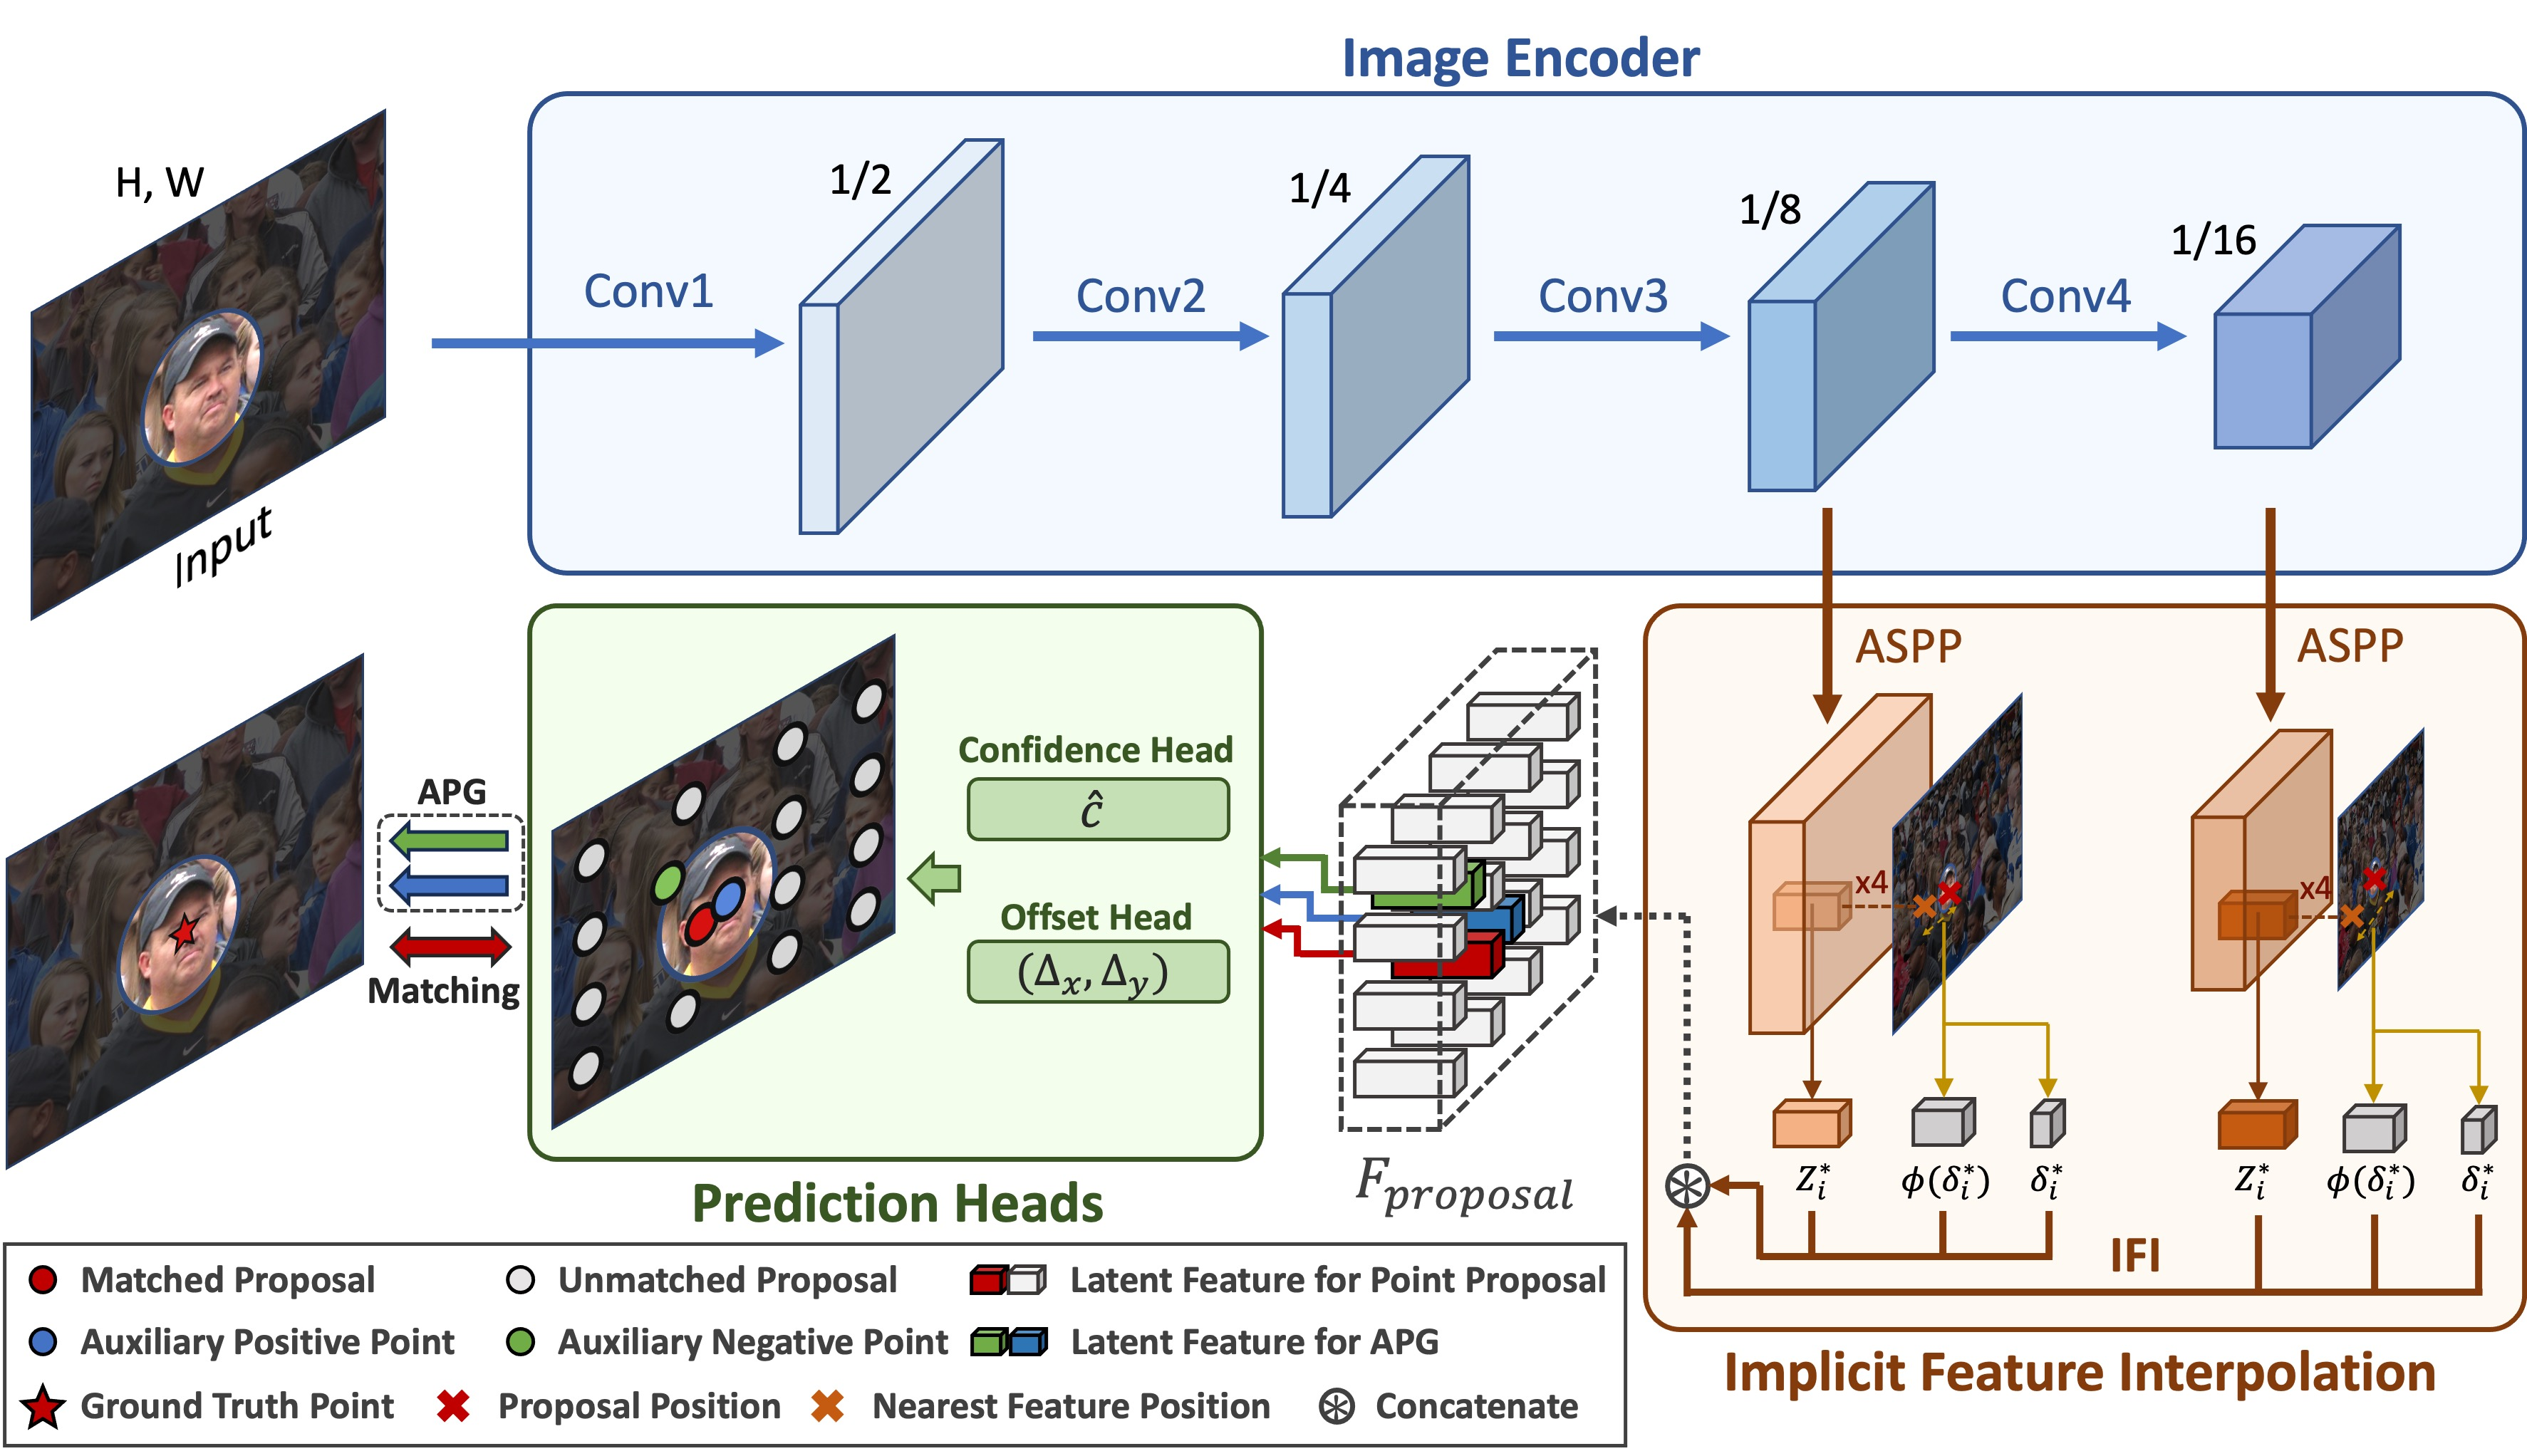
\includegraphics[width=\linewidth]{figures/apgcc_arch}
    \caption{APGCC 整体架构（引自原论文）。图像编码器提取 $1/2$--$1/16$ 多尺度特征，
    IFI（Implicit Feature Interpolation）在连续坐标上隐式插值特征，预测头为每个锚点输出
    置信度 $\hat{c}$ 与坐标偏移 $(\Delta_x,\Delta_y)$，再经匈牙利匹配与真值点一对一关联。
    本次 baseline 采用其编码器、IFI 与预测头主干；图中辅助点引导（APG）分支在 baseline
    中未启用（\texttt{AUX\_EN=False}）。}
    \label{fig:apgcc-arch}
\end{figure}

\begin{figure}[H]
    \centering
    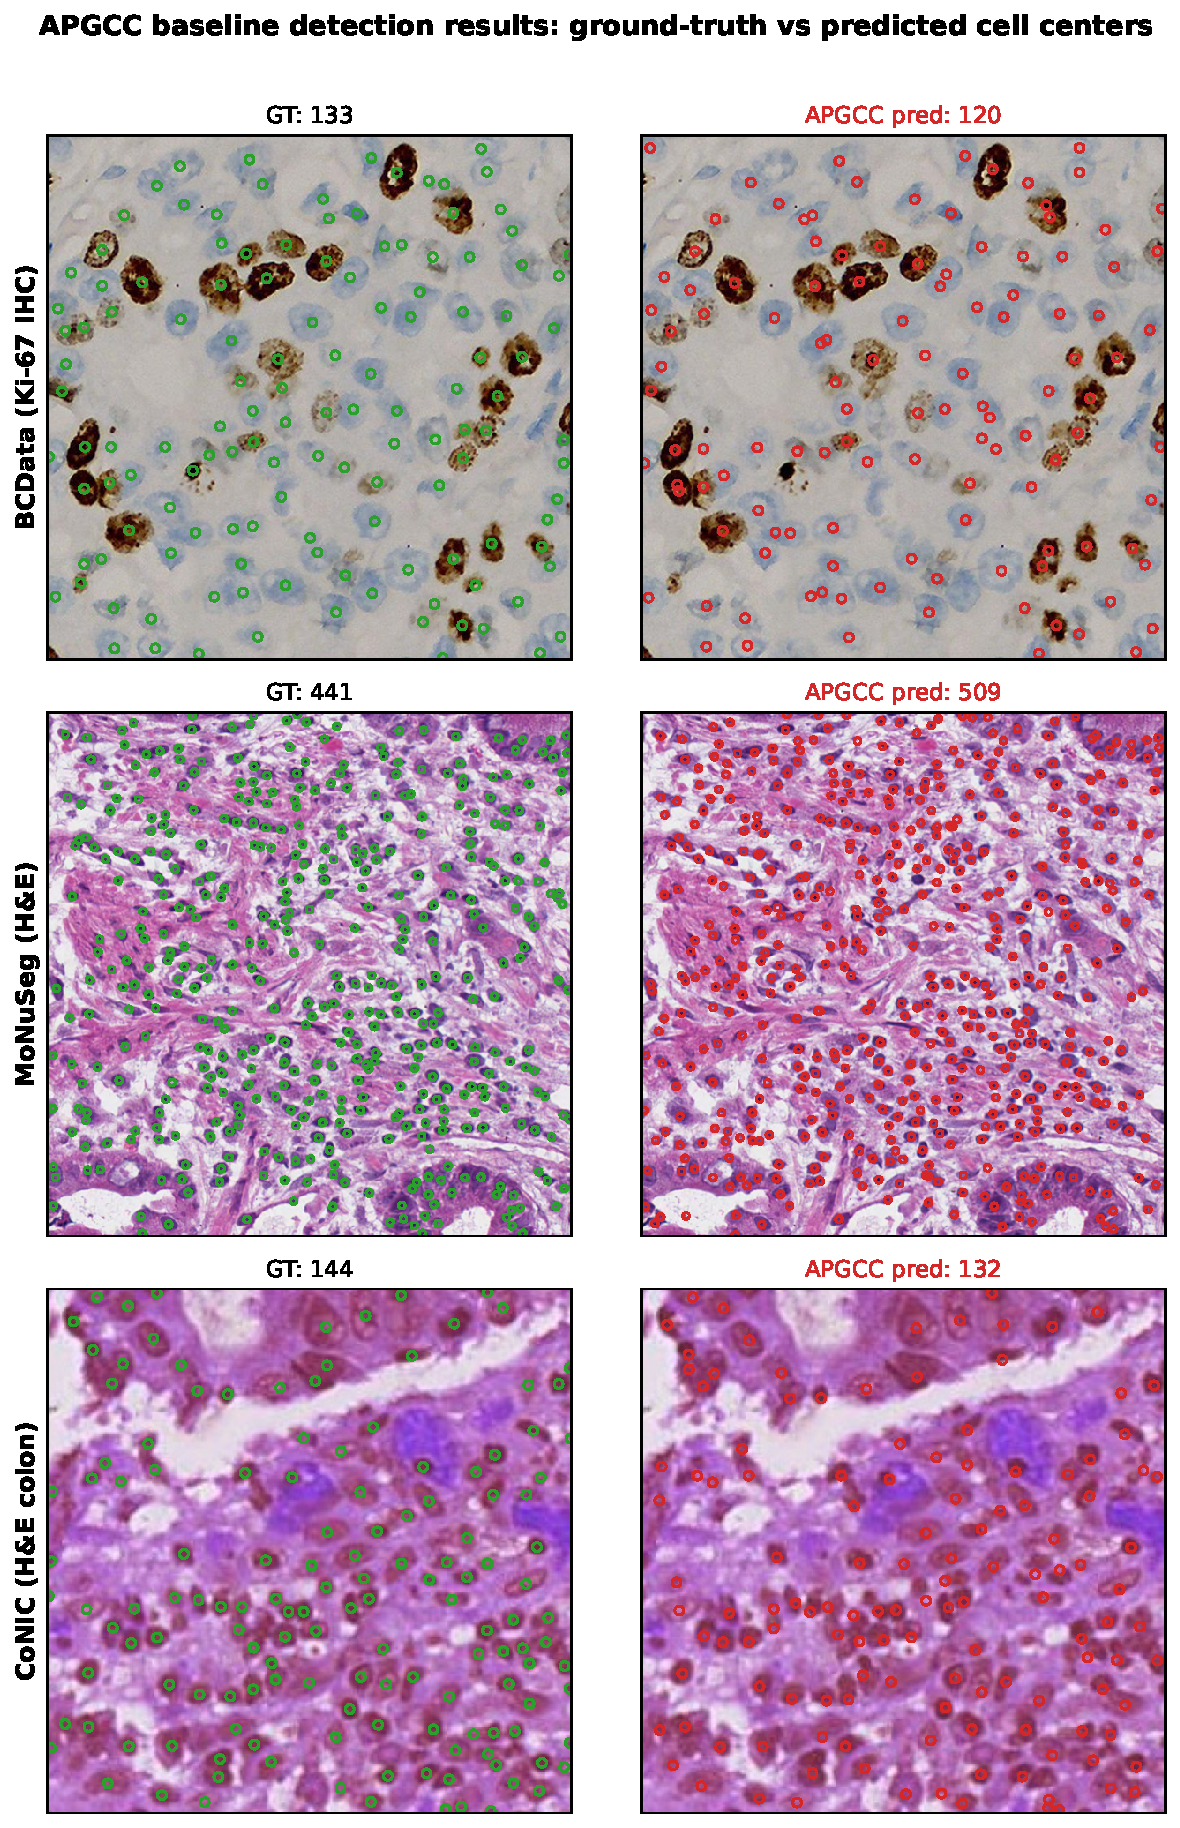
\includegraphics[width=0.74\linewidth]{figures/fig_baseline_detection}
    \caption{APGCC baseline 在三个数据集测试集上的检测结果（代表性整图）。每行一个数据集，
    左列为真值中心点（绿）、右列为 APGCC 预测中心点（红），标题给出对应计数。
    BCData（GT\,$133$/预测\,$120$）、MoNuSeg（GT\,$441$/预测\,$509$）、CoNIC（GT\,$144$/预测\,$132$）
    的预测中心点均与细胞分布吻合，表明点监督框架可直接迁移到病理细胞中心定位与计数。}
    \label{fig:apgcc-detection}
\end{figure}

\begin{figure}[H]
    \centering
    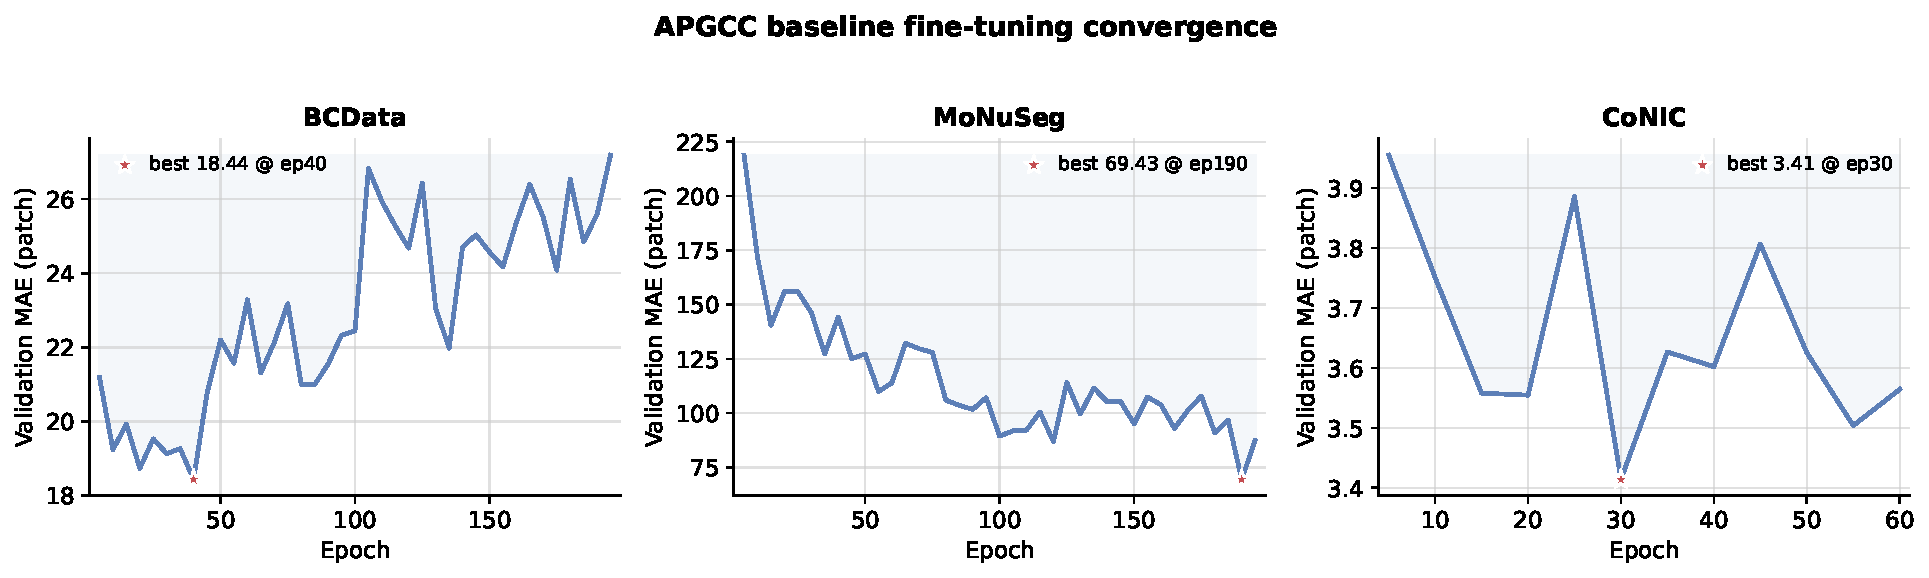
\includegraphics[width=\linewidth]{figures/fig_train_curves}
    \caption{三数据集 baseline 微调的验证 MAE 收敛曲线（红点为最佳轮）。BCData 早收敛后过拟合，
    MoNuSeg 慢且波动，CoNIC 快速收敛——反映尺度/裁剪差异对训练稳定性的影响。}
    \label{fig:apgcc-curve}
\end{figure}

\begin{figure}[H]
    \centering
    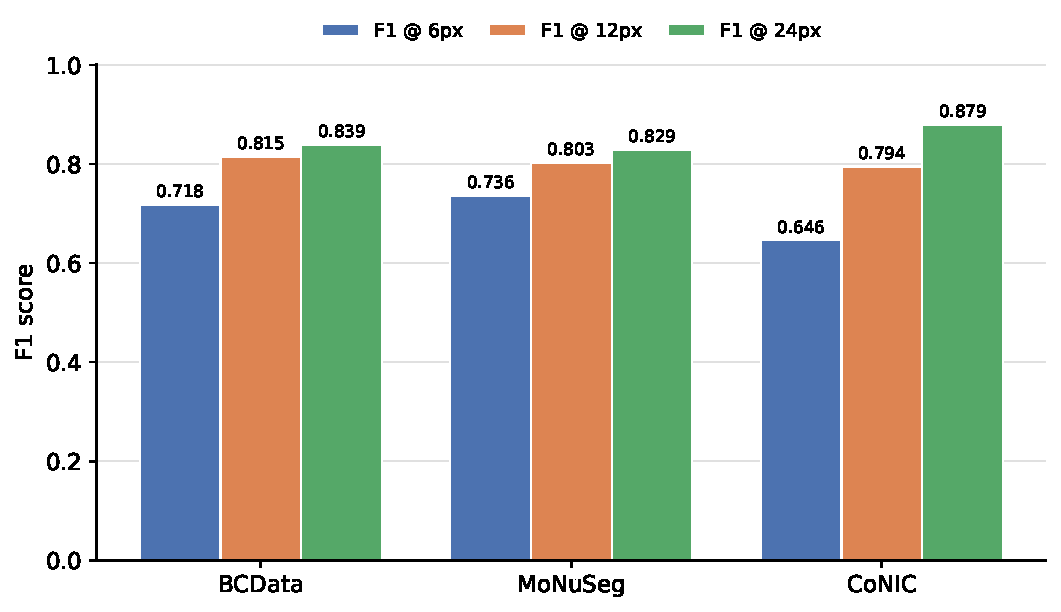
\includegraphics[width=0.74\linewidth]{figures/fig_localization_f1}
    \caption{三数据集 baseline 定位 F1@6/12/24\,px 对比。随匹配半径放宽 F1 提升；
    CoNIC 在 $6$\,px 下最低，体现密集小目标精确定位之难。}
    \label{fig:apgcc-f1}
\end{figure}

\begin{figure}[H]
    \centering
    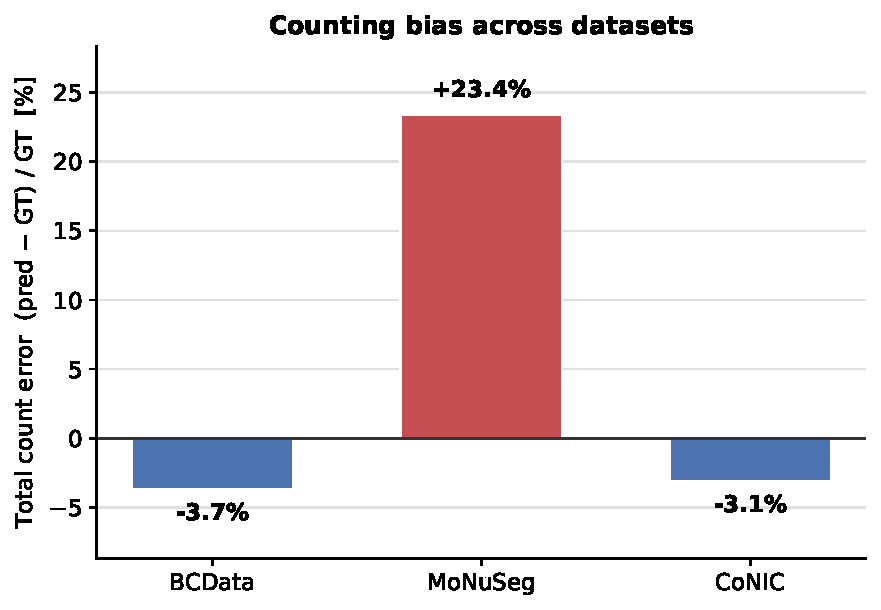
\includegraphics[width=0.62\linewidth]{figures/fig_counting_bias}
    \caption{三数据集 baseline 计数偏差（预测总数相对真值）。MoNuSeg 高密度粘连导致显著过计数，
    BCData/CoNIC 轻微欠计数，说明固定阈值难以适配不同密度分布。}
    \label{fig:apgcc-bias}
\end{figure}

\begin{figure}[H]
    \centering
    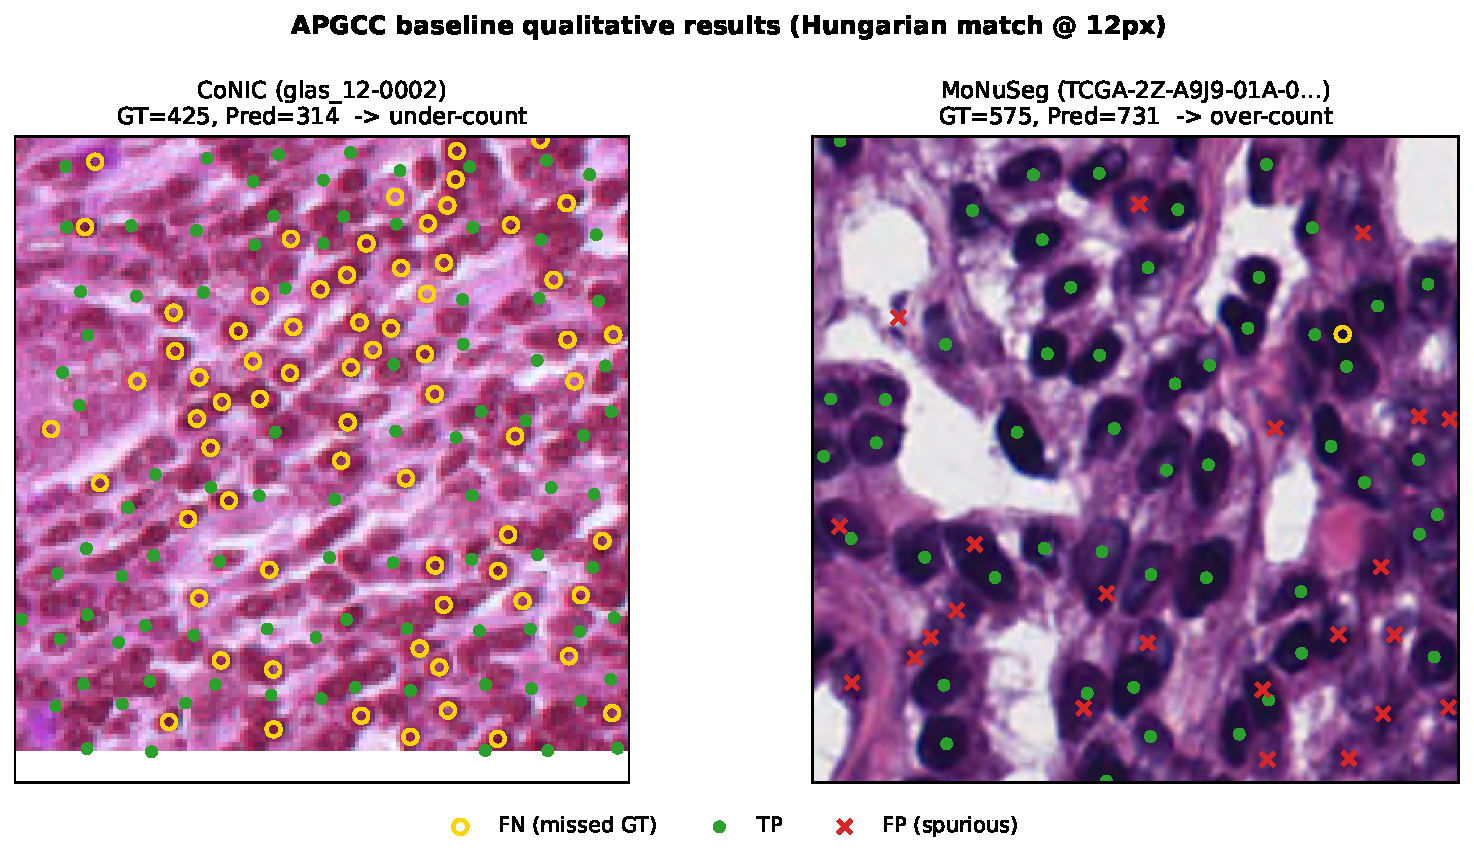
\includegraphics[width=\linewidth]{figures/fig_qualitative}
    \caption{APGCC baseline 定性结果（匈牙利匹配 @ $12$\,px；绿点为 TP、红叉为 FP、黄圈为漏检的 GT）。
    左：CoNIC 密集 patch（\texttt{glas\_12-0002}，GT $425$ / 预测 $314$），密集小目标存在大量漏检，
    对应\emph{欠计数}；右：MoNuSeg 细胞核粘连区（GT $575$ / 预测 $731$），相邻核被重复响应而产生假阳性，
    对应\emph{过计数}。二者直观印证了密度相关的计数偏差。}
    \label{fig:apgcc-qual}
\end{figure}


\section*{困难样本诊断与各方向改进}
% =============================================================================
% APGCC 困难样本诊断 + 参考点诊断与置信度--匹配校准改进方法与实验结果(仅 A 部分)
% 依赖宏包: graphicx, booktabs, amsmath, float, multirow, tabularx
% 需 \graphicspath{{figures/}}
% =============================================================================

\subsection{APGCC困难样本诊断}

本文选择APGCC作为后续优化模型，并不是因为其在所有数据集和所有指标上均达到最优，而是因为APGCC直接输出细胞中心点，与本课题的统一点匹配评估、区域计数和错误可视化协议一致。为了明确APGCC后续应该优化什么，本文在确定APGCC为主线模型后，对其在三个统一测试集上的困难样本进行诊断分析。对每张测试图像，记真实点数为$N_i$，预测点数为$\hat{N}_i$，计数误差为$e_i=\hat{N}_i-N_i$。困难样本按照$|e_i|$排序选取，同时保留显著少计和显著多计样本；定位误差采用$12$像素半径进行一对一匹配，统计TP、FP和FN。可视化时先将图像划分为$4\times4$区域，计算每个区域的$\hat{N}-N$，再裁取绝对区域误差最大的局部区域，用于观察漏检、误检和重复响应的空间分布。

\begin{table}[htbp]
    \centering
    \caption{APGCC在三个测试集上的困难样本统计依据}
    \label{tab:apgcc-hard-summary}
    \scriptsize
    \resizebox{\linewidth}{!}{
    \begin{tabular}{lrrrrrrrrr}
        \toprule
        数据集 & 样本数 & GT总数 & Pred总数 & 总误差 & MAE$\downarrow$ & MSE$\downarrow$ & Precision$\uparrow$ & Recall$\uparrow$ & F1$\uparrow$ \\
        \midrule
        CoNIC & 991 & 112545 & 88094 & $-21.73\%$ & 25.50 & 1395.13 & 0.898 & 0.703 & 0.789 \\
        BCData & 402 & 65432 & 61815 & $-5.53\%$ & 19.13 & 608.67 & 0.836 & 0.790 & 0.813 \\
        MoNuSeg & 14 & 6697 & 8018 & $+19.73\%$ & 94.36 & 9781.07 & 0.756 & 0.905 & 0.824 \\
        \bottomrule
    \end{tabular}}
\end{table}

\begin{figure}[htbp]
    \centering
    \includegraphics[width=\linewidth]{figures/apgcc_hard_three_dataset_representative_zoom.png}
    \caption{APGCC代表性困难样本局部可视化。三行从上至下分别为CoNIC、BCData和MoNuSeg；三列从左至右分别为真实中心点、APGCC预测中心点和12像素匹配下的TP/FP/FN结果。绿色表示TP或真实点，红色表示预测点或FP，黄色表示FN。}
    \label{fig:apgcc-hard-three-dataset}
\end{figure}

由表~\ref{tab:apgcc-hard-summary}和图~\ref{fig:apgcc-hard-three-dataset}可以得到三点结论。第一，APGCC在CoNIC上存在最明确的系统性少计，预测总数比GT低$21.73\%$，Recall仅为$0.703$，说明高密度结肠细胞核区域中大量真实中心点没有被保留下来。第二，BCData同样存在少计，但总误差仅为$-5.53\%$，其困难样本主要集中在局部密集重叠和阳性/阴性外观差异明显的区域，问题强度弱于CoNIC。第三，MoNuSeg的错误方向与前两者不同，整体为$+19.73\%$过计，Precision下降到$0.756$，说明在跨器官H\&E图像中APGCC更容易产生重复点或背景误检。因此，APGCC后续优化不能只依赖单一平均指标，而应同时观察总预测偏差、Recall、Precision以及困难样本中的TP/FP/FN空间分布。

上述诊断表明，APGCC 的误差并非单一方向，而是随数据特性呈现少计（CoNIC $-21.7\%$、Recall $0.70$）、
过计（MoNuSeg $+19.7\%$）与密集粘连重复等不同失败模式。本文聚焦其中最突出、且与本课题高密度细胞计数
最相关的\emph{高密度区系统性少计}，从参考点数量诊断与置信度--匹配校准入手提出改进，下节完整汇报其诊断、
配方消融、机理特异性迁移与基座依赖性分析。

% =============================================================================
\subsection{改进方法与实验结果：参考点诊断与置信度--匹配校准}
% =============================================================================

\paragraph{诊断先行：参考点不是瓶颈。}
方向 A 的初始假设是 APGCC 在密集区域 proposal 覆盖不足，可通过将每网格参考点由 $K{=}4$ 增至 $K{=}8$ 缓解。
为验证该假设，本文先做不训练的 Phase~0 诊断：统计每个真实核 $12$\,px 邻域内是否存在候选点。结果显示
\emph{无候选点比例为 $0\%$}，即每个真核附近都已有提议点，proposal 覆盖并非瓶颈。进一步实验表明
（表~\ref{tab:A-ablation}、图~\ref{fig:A-ablation}），直接加 $K{=}8$ 不仅无益，反而把 CoNIC 的 MAE
从 $25.50$ 抬高到 $32.66$，是一个明确的\emph{负结果}。诊断由此定位到两个真实原因：
（i）\emph{匹配争用}——$90\%$ 真核旁存在高分候选，但一对一匈牙利匹配加无去重，使密集区互相抢点，Recall 仅 $0.70$；
（ii）\emph{置信度被类别不平衡压保守}——候选点数（约 $10^3$）远多于真核数（约 $10^2$），负样本主导分类损失，
正样本置信度被系统性压低。因此正确方向不是\emph{加候选点}，而是\emph{校准匹配与置信度}。

\paragraph{对症配方：EOS$\downarrow$ + $\tau\uparrow$ + focal + 密度自适应阈值。}
针对上述两因，方向 A 在统一增强（unified）基座上逐机理叠加四项改动，并保持单变量可归因：
降低无目标类权重 \texttt{EOS\_COEF}（缓解负样本主导）、提高匹配代价 \texttt{SET\_COST\_POINT}（$\tau$，
缓解密集区抢点）、引入 softmax-focal（对易分负样本降权）、以及推理期按局部密度自适应选阈值。
逐步消融见表~\ref{tab:A-ablation} 与图~\ref{fig:A-ablation}：降低 EOS 与提高 $\tau$ 已恢复大部分增益——
\textbf{EOS0.10\,+\,$\tau$0.10} 将 CoNIC 的 MAE 由 $25.50$ 降到 $14.00$（$-45\%$），并把计数偏差由
$-21.7\%$ 收敛到 $+0.2\%$、F1 升到 $0.786$；在此之上叠加 focal 把 MAE 进一步压到 \textbf{13.44}（$-47\%$），
但以轻微定位代价换取（F1 $0.786\!\to\!0.761$）；推理期密度自适应阈值在该（已较平衡的）基座上几乎无额外增益
（$13.44\!\to\!13.54$）。总体而言，unified 上的对症校准把 MAE 从 $25.50$ 降到 $\approx13.4$（$-47\%$），增益主要由
EOS/$\tau$ 贡献，focal 边际有效、密度自适应在此基座近似中性。

\paragraph{模块改动的具体实现。}
上述四项均为对 APGCC 原有损失/匹配/推理的\emph{定点修改}，改动量、默认值与数学形式如下，以便复现。

\textbf{(i) 降低无目标类权重 \texttt{EOS\_COEF}。}
APGCC 的 proposal 分类损失是二类（前景/无目标）加权交叉熵：前景（正样本）权重固定为 $1$，
无目标类（负样本）权重记为 $\lambda_1{=}\texttt{EOS\_COEF}$（即下式~\eqref{eq:A-focal-cls} 中的 $\lambda_1$）。
基线 $\texttt{EOS\_COEF}{=}0.5$。密集图中候选点（约 $10^3$）远多于真核（约 $10^2$），
负样本主导该损失、把前景置信度系统性压保守。改动只是把 $\lambda_1$ 由 $0.5$ 降到 $0.10$（unified），
相对上调前景类梯度，提升密集区正样本置信度与 Recall（对应 \texttt{APGCC.py} 中 \texttt{empty\_weight[0]=eos\_coef}）。

\textbf{(ii) 提高匹配代价 $\tau$（\texttt{SET\_COST\_POINT}）。}
训练用一对一匈牙利匹配，其代价矩阵为
$C=\tau\cdot\lVert \hat{p}-p\rVert_{2}-\lambda_{\text{cls}}\cdot\hat{c}$（$\hat{c}$ 为提议点的前景置信度），
$\tau{=}\texttt{SET\_COST\_POINT}$ 是坐标 $L_2$ 距离项的权重，$\lambda_{\text{cls}}{=}\texttt{SET\_COST\_CLASS}{=}1$。
基线 $\tau{=}0.05$，几何项过弱，密集区多个真核会去抢同一个高分候选（\emph{匹配争用}）。改动把 $\tau$ 由 $0.05$ 提到
$0.10$/$0.35$，加大"谁离得近"在匹配中的权重，缓解抢点。注意 $\tau$ \emph{只改匹配、不改损失函数本身}（\texttt{matcher.py}）。

\textbf{(iii) softmax-focal（\texttt{FOCAL\_GAMMA}）。}
基线为上面的加权 CE。改动对每个 proposal 的分类损失乘上 focal 调制因子：正样本（前景）乘 $(1-\hat{c})^{\gamma}$、
负样本（背景）乘 $\hat{c}^{\gamma}$，$\gamma{=}\texttt{FOCAL\_GAMMA}$，对"已分对的易样本"（该因子 $\to 0$）降权，
把梯度进一步集中到难样本、抑制易分背景主导；完整形式见下式~\eqref{eq:A-focal-cls}。$\gamma{=}0$ 时因子恒为 $1$、
严格退化回原加权 CE，可无缝开关（\texttt{APGCC.py:118--126}）。

\textbf{(iv) 密度自适应阈值（\texttt{density\_threshold.py}）。}
基线推理用\emph{单一全局}分数阈值（$0.5$）决定保留哪些候选点。诊断发现越密的图最优阈值越低
（$\mathrm{corr}(\text{密度},\text{逐图最优阈值})<0$），因此固定阈值必然对一部分图偏错。改动是\emph{纯后处理}（模型只前向一次）：
以低参考阈值下的预测点数 $\text{pred\_count}@\text{ref}$ 作为测试时可得的密度信号，把测试图按密度分为 $\text{nbins}$（此处 $3$）档，
每档单独选一个分数阈值。为避免用测试标签作弊，档内阈值由 $2$-fold 交叉验证给出——在一折上按档选最优阈值、应用到另一折，
故所报 MAE 不含泄漏；本实验三档得到阈值 $0.55/0.5/0.5$。

\textbf{含 focal 的完整训练损失。}
沿用 P2PNet/APGCC 的点监督记法：网络输出 $M$ 个提议点 $\{(\hat{p}_j,\hat{c}_j)\}_{j=1}^{M}$，其中
$\hat{p}_j$ 为二维坐标、$\hat{c}_j\!=\!\mathrm{softmax}(\text{logit}_j)_{[1]}\!\in\![0,1]$ 为前景置信度；
真值点集为 $\{p_i\}_{i=1}^{N}$（$N\!\le\!M$）。匈牙利匹配给出 $\{1,\dots,M\}$ 上的置换 $\psi$，使前 $N$ 个
$\psi(1),\dots,\psi(N)$ 为与真值一一对应的正样本、其余 $M{-}N$ 个为负样本；置换由代价矩阵（改动 (ii)，
$\tau$ 为坐标项权重、$\lambda_{\text{cls}}{=}\texttt{SET\_COST\_CLASS}{=}1$）在正样本上最小化得到：
\begin{equation}
    \mathcal{C}(i,j)=\tau\,\lVert p_i-\hat{p}_j\rVert_2-\lambda_{\text{cls}}\,\hat{c}_j,\qquad
    \psi=\arg\min_{\psi}\;\textstyle\sum_{i=1}^{N}\mathcal{C}\big(i,\psi(i)\big).
\end{equation}
则\emph{加入 softmax-focal（改动 (iii)，指数 $\gamma\!=\!\texttt{FOCAL\_GAMMA}$）后}的分类损失为
（$\lambda_1\!=\!\texttt{EOS\_COEF}$ 为负样本权重，改动 (i)）
\begin{equation}
    \mathcal{L}_{\text{cls}}^{\text{focal}}
    =-\frac{1}{M}\left(
        \sum_{i=1}^{N}\big(1-\hat{c}_{\psi(i)}\big)^{\gamma}\log \hat{c}_{\psi(i)}
        +\lambda_1\sum_{i=N+1}^{M}\hat{c}_{\psi(i)}^{\gamma}\log\big(1-\hat{c}_{\psi(i)}\big)
    \right),
    \label{eq:A-focal-cls}
\end{equation}
其中第一项对 $N$ 个正样本、第二项对 $M{-}N$ 个负样本；$\gamma{=}0$ 时两个 focal 因子恒为 $1$，
式~\eqref{eq:A-focal-cls} 严格退化为 APGCC 原有的加权交叉熵。匹配点对的坐标回归损失不变：
\begin{equation}
    \mathcal{L}_{\text{loc}}=\frac{1}{N}\sum_{i=1}^{N}\big\lVert p_i-\hat{p}_{\psi(i)}\big\rVert_2^2 .
\end{equation}
方向 A 关闭辅助分支（$\texttt{loss\_aux}$ 权重为 $0$），故完整训练目标为二者加权和
\begin{equation}
    \mathcal{L}=\mathcal{L}_{\text{cls}}^{\text{focal}}+\lambda_{\text{loc}}\,\mathcal{L}_{\text{loc}},
    \qquad \lambda_{\text{loc}}=\texttt{POINT\_LOSS\_COEF}=2\times10^{-4}.
\end{equation}
改动 (i)/(ii)/(iii) 分别作用于负样本权重 $\lambda_1$、匹配代价中的 $\tau$、以及 focal 指数 $\gamma$；改动 (iv) 只在推理期作用、不进入 $\mathcal{L}$。

\begin{table}[H]
    \centering
    \caption{方向 A 配方逐步消融（CoNIC 测试集，unified 基座）。末行"密度自适应阈值"为
    \texttt{density\_threshold.py} 的 2-fold 交叉验证，按密度分档逐图赋阈值（此处三档 $0.55/0.5/0.5$），
    其 MSE/Recall/F1 经统一 \texttt{centroid\_eval.py} 在分档阈值下的预测点上重新评测得到，口径与其余行一致。
    所有行均取各自训练的\emph{最终 val-best 检查点}（诚实模型选择）。}
    \label{tab:A-ablation}
    \small
    \begin{tabular}{lcccccc}
        \toprule
        配方 & 阈值 & MAE$\downarrow$ & MSE$\downarrow$ & Recall$\uparrow$ & F1@12$\uparrow$ & 计数偏差 \\
        \midrule
        APGCC baseline            & 0.50 & 25.50 & 1395 & 0.703 & 0.789 & $-21.7\%$ \\
        $K{=}8$（负结果）          & 0.50 & 32.66 & 2029 & 0.659 & 0.768 & $-28.5\%$ \\
        \quad +\,EOS\_COEF$\downarrow$ & 0.10 & 15.19 & 670  & 0.738 & 0.762 & $-6.3\%$ \\
        \quad +\,$\tau\uparrow$（匹配代价） & 0.35 & 14.00 & 513  & 0.787 & 0.786 & $+0.2\%$ \\
        \quad +\,focal（易负降权）  & 0.50 & \textbf{13.44} & 532  & 0.747 & 0.761 & $-3.8\%$ \\
        \quad +\,密度自适应阈值     & 密度分档 & 13.54 & 534  & 0.745 & 0.762 & $-4.5\%$ \\
        \bottomrule
    \end{tabular}
\end{table}

\begin{figure}[H]
    \centering
    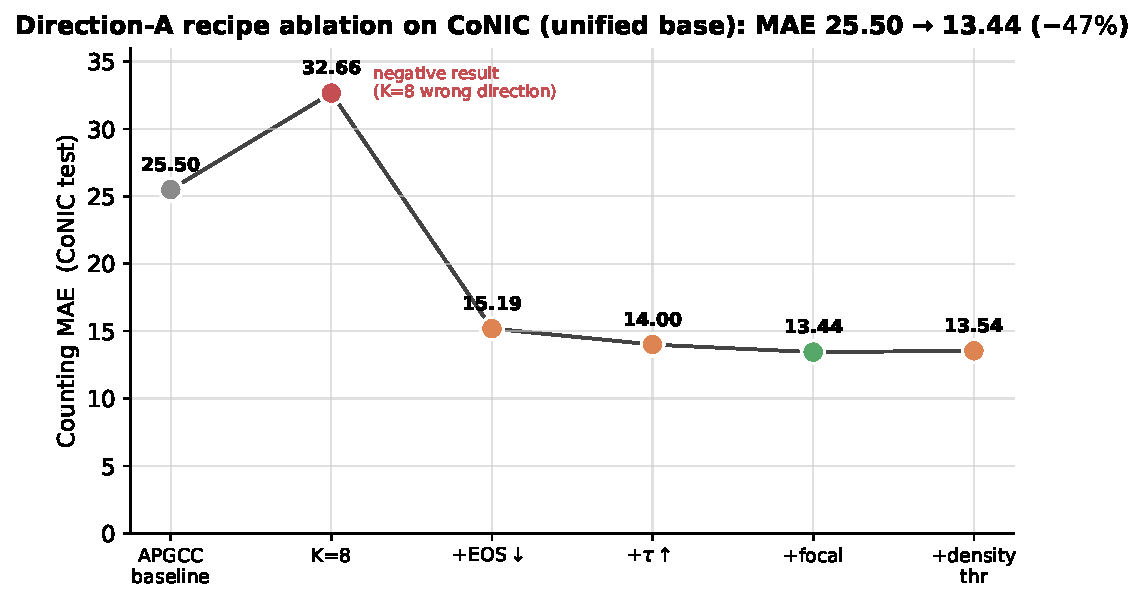
\includegraphics[width=0.82\linewidth]{figures/fig_A_ablation}
    \caption{方向 A 在 CoNIC（unified 基座）上的配方逐步消融（均为最终 val-best 检查点）。灰点为 baseline，
    红点为 $K{=}8$ 负结果，绿点为最优配方；MAE 由 $25.50$ 降至 $13.44$（$-47\%$），主要由 EOS/$\tau$ 贡献。}
    \label{fig:A-ablation}
\end{figure}

\paragraph{机理特异性：配方精准修复"少计"，对其它失败模式中性。}
为验证该配方是\emph{对症}而非碰运气，方向 A 在三个数据集上各自训练并对比（表~\ref{tab:A-transfer}、
图~\ref{fig:A-transfer}）。结果与各数据集的失败模式高度吻合：CoNIC（密集少计）大幅获益（$25.50\to14.00$）；
BCData（计数平衡）近似中性（$17.19\to18.35$）；MoNuSeg（整体过计）近似中性（$26.21\to24.79$）。
即该配方只在"少计"这一失败模式上显著生效，对"平衡"和"过计"模式不强行改变，符合其机理设计。

\begin{table}[H]
    \centering
    \caption{方向 A 配方的三数据集机理特异性迁移（各自训练）}
    \label{tab:A-transfer}
    \small
    \begin{tabular}{lcccc}
        \toprule
        数据集 & 失败模式 & baseline MAE & +配方 MAE & 结论 \\
        \midrule
        CoNIC   & 密集少计 & 25.50 & 14.00 & 大幅获益 \\
        BCData  & 平衡     & 17.19 & 18.35 & 近似中性 \\
        MoNuSeg & 过计     & 26.21 & 24.79 & 近似中性 \\
        \bottomrule
    \end{tabular}
\end{table}

\begin{figure}[H]
    \centering
    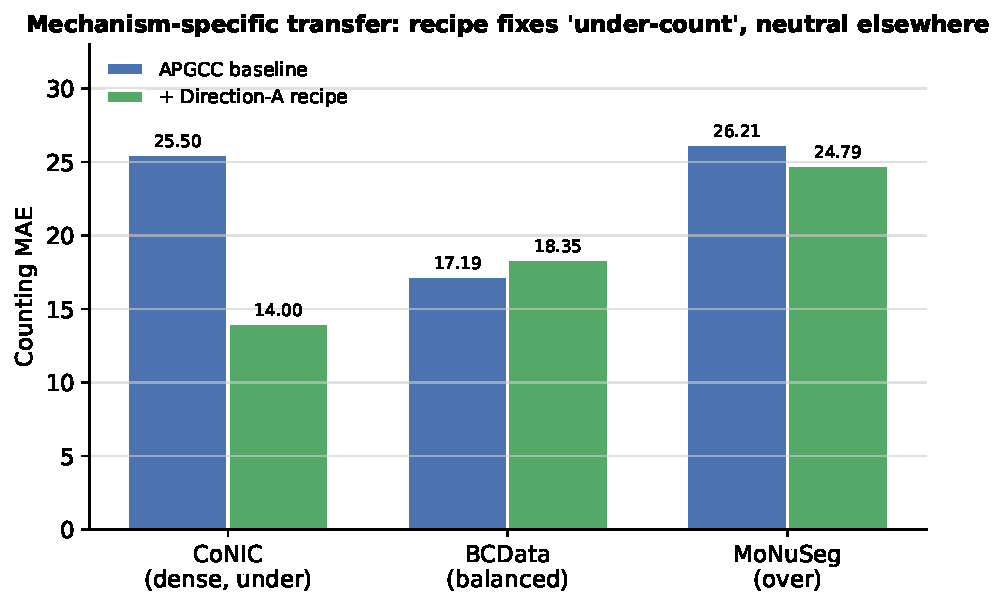
\includegraphics[width=0.74\linewidth]{figures/fig_A_transfer}
    \caption{方向 A 配方在三数据集上的迁移。仅 CoNIC（密集少计）显著获益，BCData/MoNuSeg 近似中性，
    印证配方对"少计"失败模式的针对性。}
    \label{fig:A-transfer}
\end{figure}

\paragraph{基座依赖性：native 是最终落地基座，校准价值正比于基座标定误差。}
方向 A 的最终落地基座是\emph{原生增强（native）}——团队后续所有改进与集成均在 native 上进行，
统一增强（unified）仅作为"增广敏感性 / 机理验证"的对照保留。两套增强对 CoNIC 的影响差异巨大：
unified 严重伤害 CoNIC（unified baseline MAE $25.50$，而统一 native baseline 仅 $12.93$，相差近一倍），
其根源是 unified 把置信度分布推向严重欠预测，而 native 基座本身已较平衡（计数偏差约 $-5.5\%$）。
因此本文把方向 A 的\emph{完整 EOS$\times\tau$ 与 focal 扫描}放在 native 基座上、并\emph{训练至收敛}
（ep$\ge$120）后报告，结果见表~\ref{tab:A-native} 与图~\ref{fig:A-native}。

native 上的扫描呈现三点与 unified \emph{相反}的规律。其一，所有配方的 MAE 都落在 $10.5$--$16.3$、
与统一 native baseline（$12.93$）处于同一量级，没有 unified 上那种量级改善。其二，最优方向与 unified 完全相反——
native 上 EOS 越低越差（$0.25\!\to\!10.83$，$0.10\!\to\!12.50$，$0.05\!\to\!16.31$），而 unified 上恰是
EOS 越低越好；$\tau$ 过大（$0.15$）同样劣化。其三，就真正关心的定位 F1 而言，\emph{统一 baseline 的 $0.7929$
即为全表最佳，没有任何 A 配方能超过它}（最接近的 EOS$0.25/\tau0.10$ 也仅 $0.78$ 量级）；尤其
EOS$0.10/\tau0.05$ 虽在低阈值（$0.1$）下取得全表最低 MAE $10.54$，但其 F1 仅 $0.7185$，说明该点是靠
\emph{正负误差相消}得到的好计数、定位质量反而最差——只看单一 MAE 会产生误导。focal 在 native 同样无益（$12.15$）。
综合 MAE 与 F1：native 上 A 配方至多在计数上与 baseline 互有胜负，但\emph{定位始终不及 baseline}，整体呈中性偏弱。

由此得到方向 A 的核心结论：\emph{置信度与匹配校准的价值，正比于基座本身的标定错误程度}。在标定很差的
unified 基座上，校准把 MAE 从 $25.50$ 拉到 $\approx13.4$（$-47\%$，转化巨大）；而在标定良好的 native 基座上，
同类校准增益显著温和、远小于 unified（图~\ref{fig:A-native} 右），且定位 F1 始终不及 baseline。两基座上最优超参方向相反，
恰恰说明该方法是\emph{对症校准}而非偶然调参——native 基座已经"健康"，可校准的空间本就很小。

\begin{table}[H]
    \centering
    \caption{方向 A 在 native（最终落地）基座上的 EOS$\times\tau$ 与 focal 完整扫描
    （CoNIC 测试集，均训练至 ep$\ge$120 收敛；阈值取各配置 MAE 甜点）。baseline 行采用\emph{团队统一 native
    baseline}（CoNIC 方向E 口径，MAE $12.93$/F1 $0.7929$），与各 A 配置非同次运行，故 MAE 的细微差异含运行间方差，
    \emph{稳健结论以定位 F1 为准}（无 A 配置超过 baseline）。}
    \label{tab:A-native}
    \small
    \begin{tabular}{lcccccl}
        \toprule
        native 配置 & 阈值 & MAE$\downarrow$ & MSE$\downarrow$ & F1@12$\uparrow$ & 计数偏差 & 备注 \\
        \midrule
        baseline（统一口径）           & 0.50 & 12.93 & 468.9  & \textbf{0.7929} & $-5.5\%$ & 团队统一 native baseline（定位最优） \\
        EOS0.25/$\tau$0.10             & 0.40 & 10.83 & 396.9  & 0.7810 & $-1.3\%$ & native MAE 最优 \\
        \quad（同配置 @0.50）           & 0.50 & 11.12 & 438.8  & 0.7799 & $-4.6\%$ & 阈值敏感性对照 \\
        EOS0.10/$\tau$0.05             & 0.10 & \textbf{10.54} & 251.6 & 0.7185 & $-0.6\%$ & 低阈值，F1 最差 \\
        EOS0.10/$\tau$0.10             & 0.70 & 12.50 & 537.1  & 0.7309 & $-2.8\%$ & $\approx$\,baseline \\
        EOS0.10/$\tau$0.15             & 0.80 & 15.10 & 398.8  & 0.7402 & $-8.5\%$ & $\tau$ 过大变差 \\
        EOS0.05/$\tau$0.10             & 0.70 & 16.31 & 1004.3 & 0.6840 & $-3.8\%$ & EOS 过低变差 \\
        +\,focal (EOS0.10/$\tau$0.10)  & 0.60 & 12.15 & 563.3  & 0.7740 & $-7.0\%$ & focal 无益 \\
        \bottomrule
    \end{tabular}
\end{table}

\begin{figure}[H]
    \centering
    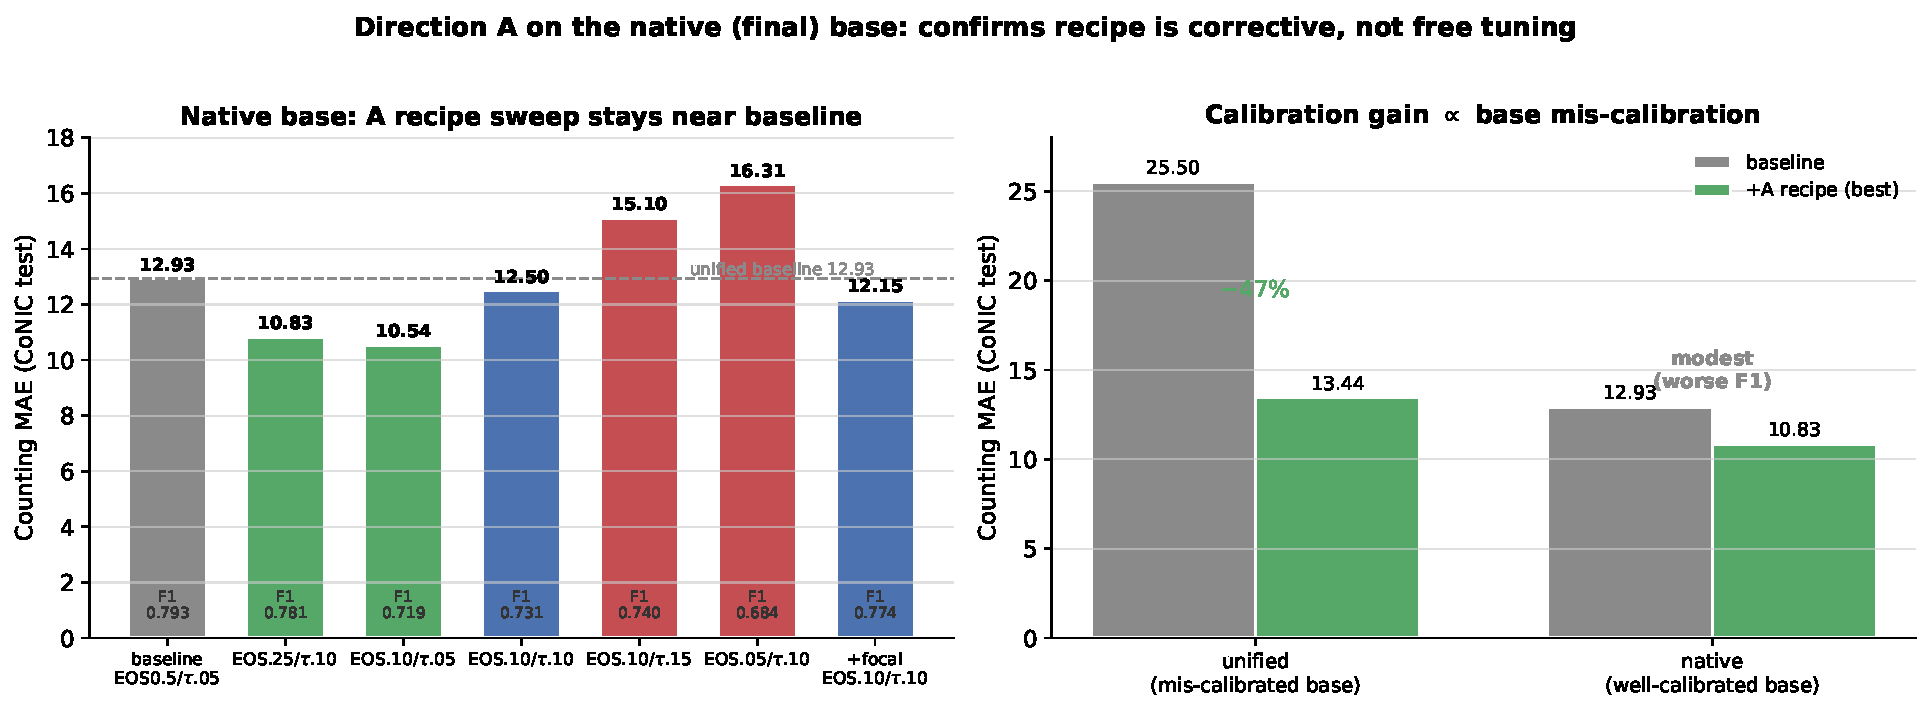
\includegraphics[width=\linewidth]{figures/fig_A_native}
    \caption{方向 A 在 native（最终落地）基座上的结果。左：EOS$\times\tau$ 与 focal 的完整扫描，
    各配方 MAE 与统一 native baseline（$12.93$）同量级、定位 F1 均不超过 baseline，且最优方向与 unified 相反；
    右：native 与 unified 的校准增益对比——unified（烂基座）转化巨大（$-47\%$），native（好基座）增益温和，
    印证"校准价值正比于基座标定误差"。}
    \label{fig:A-native}
\end{figure}

\paragraph{小结。}
方向 A 通过"先诊断、后对症"的方式，否定了直觉性的加参考点（$K{=}8$）方案，定位到匹配争用与类别不平衡
两个真因，提出 EOS$\downarrow$+$\tau\uparrow$（+focal/密度自适应）的组合校准。在标定很差的 unified 基座上，
该校准取得 MAE $25.50\to\approx13.4$（$-47\%$，主要由 EOS/$\tau$ 贡献）、计数偏差由 $-21.7\%$ 收敛到近平衡的显著改善，
作为机理验证；而在团队\emph{最终落地的 native 基座}上，由于统一 baseline（$12.93$）本身已较平衡，同类校准增益温和
（无配方在 F1 上超过 baseline、MAE 也与 baseline 同量级），最优超参方向且与 unified 完全相反。两者共同支撑方向 A 的核心结论：\emph{置信度与匹配校准是针对"少计"失败模式的
对症方法，其收益正比于基座标定误差}——这也解释了为何后续集成（见 ADE）中 A 的贡献应落在\emph{后处理校准}、
而非训练配方。


\section*{多方向集成改进}
% =============================================================================
% 多方向集成改进: ADE (完整, 真实数据) + BDC (框架)
% 依赖宏包: graphicx, booktabs, amsmath, float, multirow, tabularx
% 需 \graphicspath{{figures/}}
% 建议 \input 在"各方向改进方法与实验结果"之后.
% =============================================================================

\subsection{多方向集成改进}

在五个单方向改进各自对症一类失败模式之后，本组进一步探索将互补方向\emph{集成}，以验证
"网络结构改进、输入端增强、后处理校准"等不同层面的改进能否叠加增益。沿着困难样本诊断暴露的
两类主导问题，本组实现两条集成路线：面向\emph{形态/边缘与跨域稳定性}的 \textbf{ADE}（A$+$D$+$E），
以及面向\emph{密集漏检与粘连重复}的 \textbf{BDC}（B$+$D$+$C），见表~\ref{tab:integration-overview}。
本节完整汇报 ADE 集成（本机已完成具体实现），并给出 BDC 集成的统一框架。

\begin{table}[H]
    \centering
    \caption{两条集成路线总览}
    \label{tab:integration-overview}
    \small
    \begin{tabularx}{\linewidth}{p{0.07\linewidth}p{0.10\linewidth}Lp{0.13\linewidth}p{0.07\linewidth}}
        \toprule
        集成 & 组成方向 & 组合逻辑 & 主要数据集 & 状态 \\
        \midrule
        ADE & A $+$ D $+$ E & D（DCNv2 形变 $+$ Edge Ignore）改善形态/边缘、E（染色鲁棒增强）改善跨染色，二者共同改善\emph{训练基座}；A（密度自适应/域感知阈值校准）在不重训的\emph{后处理端}修正置信度 & CoNIC / BCData / MoNuSeg & 完整 \\
        BDC & B $+$ D $+$ C & B（密集辅助监督）提升密集区召回、D（形态/边缘结构）增强鲁棒性、C（点级排斥 $+$ 自适应去重）抑制重复点 & CoNIC / MoNuSeg & 框架 \\
        \bottomrule
    \end{tabularx}
\end{table}

% =============================================================================
\subsubsection{ADE 集成：D+E 结构改进 + A 后处理校准}

\paragraph{集成动机与组合逻辑}
病理细胞计数中，APGCC baseline 的失败模式在困难样本诊断中已定位清楚（见~\ref{tab:apgcc-hard-summary}）：
CoNIC 高密度区\emph{系统性少计}（$-21.7\%$、Recall $0.70$），MoNuSeg 跨器官 H\&E 上\emph{整体过计}
（$+19.7\%$、Precision $0.76$），二者又都受\emph{染色差异}与\emph{置信度分布偏移}的影响。A、D、E 三个方向恰好
从三个互补层面对症：D 从\emph{网络结构}（DCNv2 形变卷积让感受野自适应不规则核形态 $+$ Edge Ignore 抑制 crop
边界截断假阳性）改善形态适应与边界；E 从\emph{输入端}（病理染色鲁棒增强）提升跨染色稳定性；两者共同改善
\emph{训练基座}的表达能力与标定质量。A 则在\emph{后处理端}（密度自适应阈值、域感知阈值校准）以\emph{不重训}的
方式修正各密度/各域的置信度偏移。三者技术分工明确——D 提供更强的几何建模、E 提供染色不变性、A 在推理端做
密度/域自适应的阈值校准——互补而不重叠。就本题关注的两类病理挑战而言：\emph{细胞形态极其不规则}由 D 的 DCNv2
形变卷积直接对症——可学习采样偏移使感受野贴合近圆上皮核与细长梭形核，提升不规则核的识别；\emph{密集堆叠}在
ADE 中主要以"密集区召回 $+$ 密度自适应阈值"缓解其导致的少计（而"边界粘连"引起的相邻核合并/重复点去重，
则由互补的 BDC 方向 C 的点级排斥损失与自适应 NMS 专门处理，二者分工互补）。据此，本集成以 D 的网络为骨架、
并入 E 的 stain 增强、再叠加 A 的阈值校准，实现于 \texttt{improved/APGCC\_ADE}。

\paragraph{实现与配置}
以 D 的 APGCC 为骨架：VGG16-bn 的 conv5 末 $2$ 层标准卷积替换为 \texttt{ModulatedDeformConv2d}
（offset 零初始化，预训练权重自动映射），训练期启用 Edge band（$16$\,px、anchor 级 loss 权重
$0.1\!\to\!1.0$ 线性过渡）。E 的 pathology/stain 增强并入数据管线（亮度/对比度/颜色抖动 $+$ RGB 通道
scale-bias $+$ 轻量 blur/noise）。A 的贡献区分为两类且\emph{分别对待}：\emph{训练配方}
（EOS$\downarrow$$+$focal$+$$\tau$）折叠进 D 的 per-anchor 分类损失（保留 D 的 \texttt{sum/num\_points} 归一化）；
\emph{后处理校准}为独立的 \texttt{density\_threshold.py}（按局部密度分档赋阈，$2$-fold CV）与
\texttt{eval\_domain\_threshold.py}（每域 val 选阈$\to$test）。训练统一"从 \texttt{SHHA\_best.pth} 微调、
val 选 best、test 报"协议（conda \texttt{apgcc}，torch2.4.1+cu121）。评测用统一 \texttt{centroid\_eval.py}
在 $6/12/24$\,px 匈牙利匹配下给出计数 MAE/MSE 与定位 P/R/F1；三数据集数据根为
\texttt{/data1/llx/\{CoNICdata,BCData,MoNuSegdata\}}。

\paragraph{主结果：ADE 在设计靶点 CoNIC 上净正，迁移到另两数据集需阈值校准}
表~\ref{tab:ADE-3ds} 在三个数据集上对比 baseline 与 ADE，各给出\emph{固定阈值 $0.5$}（开箱即用）与
\emph{各自 MAE 最优阈值}（阈值校准后）两个操作点；图~\ref{fig:ADE-main-CoNIC}--\ref{fig:ADE-main-MoNuSeg}
为各数据集的对比。核心结论\emph{诚实且分数据集不同}：
（1）\textbf{CoNIC（ADE 的设计靶点，密集少计）上 ADE 真正净正}——校准后 MAE $11.31$ 优于 baseline $11.92$，
诚实 val$\to$test 全局阈值下亦有 \textbf{$11.87$}（见表~\ref{tab:ADE-module}），且 F1@12 与 baseline 持平（$0.794$）；
该净正收益来自 D+E 的结构改进（A 的密度自适应后处理经更正后无额外增益）；（2）\textbf{BCData（IHC）上 ADE 与 baseline 基本持平、略逊}（校准后 $18.92$ vs $17.38$，
F1 $0.806$ vs $0.818$）；（3）\textbf{MoNuSeg（跨器官 H\&E）上 ADE 计数更好、但定位更差}（校准后 MAE
$19.64$ vs $22.21$，而 F1@12 $0.686 < 0.779$）。因此 ADE 不是一个"三数据集一致提升"的方案，而是一个
\emph{对症密集少计}的方案：它在 CoNIC 上兑现了设计目标，迁移到形态/染色差异更大的数据集上则得失参半。
另需强调：\emph{固定 $0.5$ 下 BCData/MoNuSeg 的 ADE 数字（$28.72$/$111.93$）具有误导性}——如
表~\ref{tab:ADE-3ds} 与图~\ref{fig:ADE-thr-MoNuSeg} 所示，两个模型在这两个小/IHC 数据集上 $0.5$ 处均严重
过计（Pred/GT $1.16$--$1.23$），这是\emph{阈值假象}而非模型差异，必须做阈值校准后再比较。

\begin{table}[H]
    \centering
    \caption{ADE 主结果：三数据集 baseline vs ADE（固定 $0.5$ 与各自 MAE 最优阈值两操作点，
    统一 \texttt{centroid\_eval}；MAE/F1 为官方口径）。CoNIC 的 ADE 另有\emph{诚实} val$\to$test 全局阈值 $\mathbf{11.87}$
    （表~\ref{tab:ADE-module}；A 的密度自适应后处理经更正后无额外增益）。}
    \label{tab:ADE-3ds}
    \small
    \begin{tabular}{llcccccc}
        \toprule
        \multirow{2}{*}{数据集} & \multirow{2}{*}{方法} & \multicolumn{3}{c}{固定阈值 $0.5$} & \multicolumn{3}{c}{MAE 最优阈值} \\
        \cmidrule(lr){3-5}\cmidrule(lr){6-8}
        & & MAE$\downarrow$ & F1@12$\uparrow$ & Pred/GT & 阈值 & MAE$\downarrow$ & F1@12$\uparrow$ \\
        \midrule
        \multirow{2}{*}{CoNIC}
            & Baseline & 11.99 & 0.7944 & 0.969 & 0.45 & \textbf{11.92} & \textbf{0.7937} \\
            & ADE      & 12.25 & \textbf{0.7966} & 0.923 & 0.30 & \textbf{11.31} & 0.7938 \\
        \cmidrule{2-8}
        \multirow{2}{*}{BCData}
            & Baseline & \textbf{18.27} & \textbf{0.8145} & 0.963 & 0.45 & \textbf{17.38} & \textbf{0.8184} \\
            & ADE      & 28.72 & 0.8031 & 1.157 & 0.55 & 18.92 & 0.8062 \\
        \cmidrule{2-8}
        \multirow{2}{*}{MoNuSeg}
            & Baseline & 111.71 & \textbf{0.8032} & 1.234 & 0.80 & 22.21 & \textbf{0.7785} \\
            & ADE      & 111.93 & 0.7473 & 1.234 & 0.60 & \textbf{19.64} & 0.6858 \\
        \bottomrule
    \end{tabular}
\end{table}

\begin{figure}[H]
    \centering
    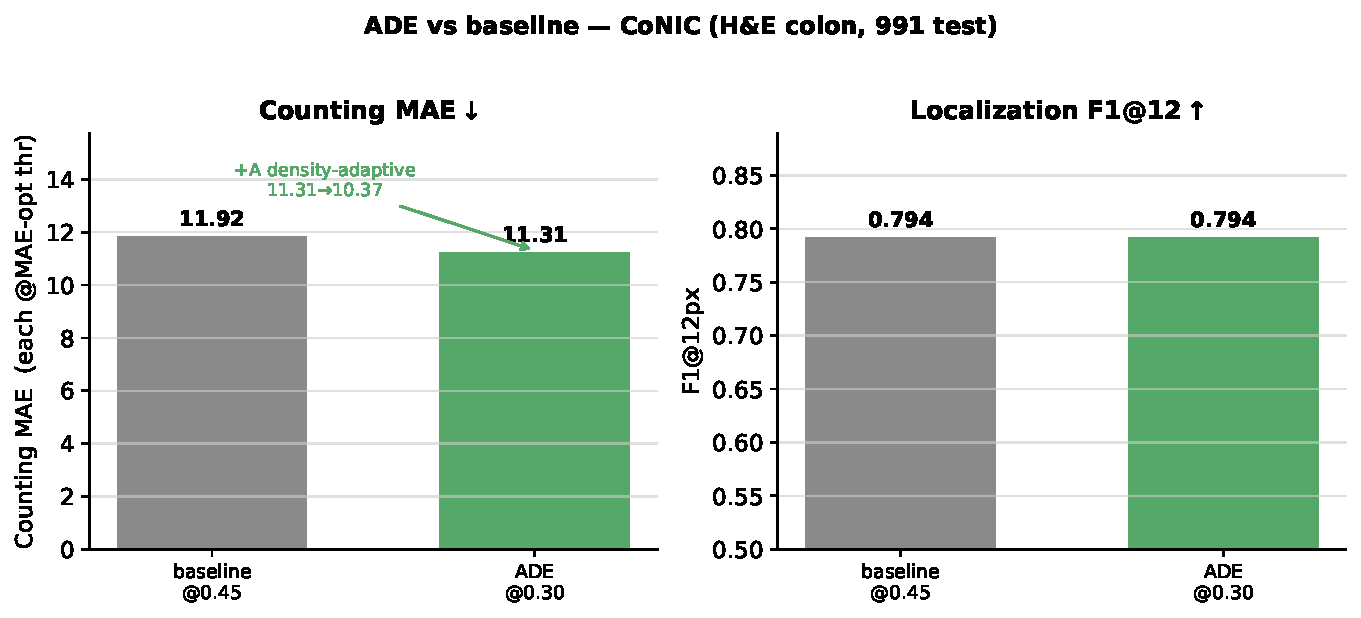
\includegraphics[width=0.72\linewidth]{figures/fig_ADE_main_comparison_CoNIC}
    \caption{ADE 主对比——CoNIC（各取 MAE 最优阈值）。MAE $11.92\!\to\!11.31$，F1@12 与 baseline 持平。
    这是 ADE 的设计靶点，D+E 结构改进带来的净正结果（密度自适应后处理经更正后无额外增益，见表~\ref{tab:ADE-module}）。}
    \label{fig:ADE-main-CoNIC}
\end{figure}

\begin{figure}[H]
    \centering
    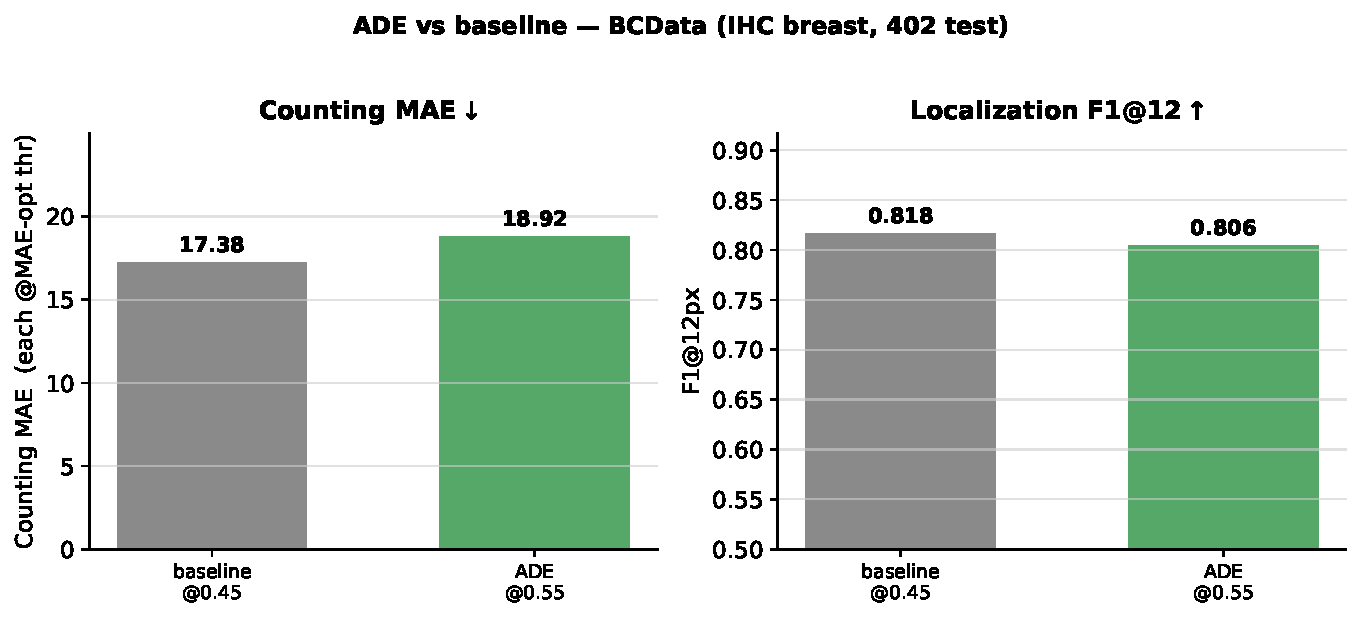
\includegraphics[width=0.72\linewidth]{figures/fig_ADE_main_comparison_BCData}
    \caption{ADE 主对比——BCData（各取 MAE 最优阈值）。ADE 与 baseline 基本持平、略逊（MAE $18.92$ vs $17.38$，
    F1@12 $0.806$ vs $0.818$）。}
    \label{fig:ADE-main-BCData}
\end{figure}

\begin{figure}[H]
    \centering
    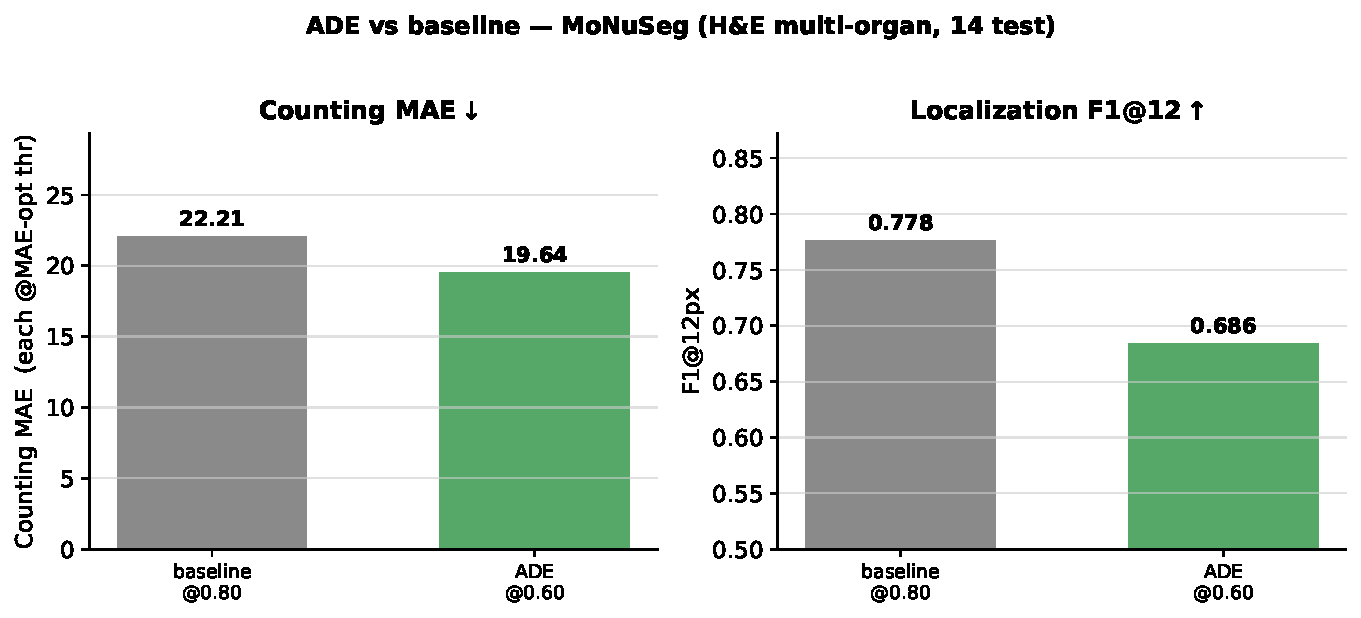
\includegraphics[width=0.72\linewidth]{figures/fig_ADE_main_comparison_MoNuSeg}
    \caption{ADE 主对比——MoNuSeg（各取 MAE 最优阈值）。ADE 计数更好（MAE $19.64$ vs $22.21$）但定位更差
    （F1@12 $0.686$ vs $0.779$）——以定位质量换计数精度。}
    \label{fig:ADE-main-MoNuSeg}
\end{figure}

\paragraph{模块贡献逐层拆解（CoNIC）：A 的"训练配方"有害、A 的"后处理"在正确 val$\to$test 协议下无净增益}
A 方向的两类贡献需\emph{区别对待}。表~\ref{tab:ADE-module} 与图~\ref{fig:ADE-module-CoNIC} 在 CoNIC 上逐层拆解：
把 A 的\emph{激进训练配方}（EOS$\downarrow$$+$focal）叠加到 D+E 基座反而有害——EOS0.10 在 $0.5$ 处过计 $+36\%$、
诚实 MAE $21.21$；EOS0.25 矫枉为欠计 $-11\%$、MAE $15.19$；二者诚实 MAE 均差于 baseline（$12.93$）。
只有\emph{关闭}A 的训练配方、仅保留 D+E 结构改进的 \textbf{D+E clean} 版，才达到并超过 baseline（fixed$0.5$
MAE $12.25$、val$\to$test 全局阈值 $0.45$ 下 \textbf{$11.87$}、F1@12 $\mathbf{0.7966}$）——这是 ADE 在 CoNIC 上的
\emph{主结果}，其净正收益完全来自 D+E 的结构改进。\emph{（更正）}A 的密度自适应后处理\emph{并不带来额外增益}：
早前所报 $10.37$（$\Delta{=}{+}1.0$）是把分档阈值\emph{在测试集上}用 $2$-fold CV 选出的\emph{泄漏}结果，非合法协议。
按正确协议在 \emph{val} 上拟合分档边界与每档阈值（$0.4/0.45/0.5$）、冻结后套用到 test，密度分档 MAE 为 $12.27$，
反而比单一 val 全局阈值 $11.87$ \emph{差 $0.39$}；且 val 拟合出的"越密阈值越高"与测试集上"越密越低"（$0.5/0.3/0.1$）
方向相反，说明该密度信号不稳定、不可迁移。逐图 oracle 上界 $5.63$（不可达）。
（注：BCData/MoNuSeg 上未做 D-only / D+E-clean 变体训练，故逐层拆解仅在 CoNIC 上给出。）

\begin{table}[H]
    \centering
    \caption{ADE 模块逐层拆解（CoNIC test，GT $112545$）。MAE 均为\emph{诚实} val$\to$test：全局阈值行的阈值、
    以及密度分档行的分档边界与每档阈值，全部在 val 上选定后冻结、原样套用到 test（不使用任何测试集标签调参）。
    密度分档一行为\emph{更正结果}——不再带来增益（$12.27>11.87$，F1 未重评）；逐图 oracle 为不可达上界。}
    \label{tab:ADE-module}
    \small
    \begin{tabular}{llccl}
        \toprule
        配置 & 阈值策略 & MAE$\downarrow$ & F1@12$\uparrow$ & 说明 \\
        \midrule
        APGCC baseline（统一参照）   & $0.5$          & 12.93 & 0.793 & 团队统一 native baseline \\
        ADE / EOS0.10（激进配方）    & val$\to$test   & 21.21 & 0.777 & 过计 $+36\%$；A 密度自适应 $\Delta{=}0$ \\
        ADE / EOS0.25（温和配方）    & val$\to$test   & 15.19 & 0.783 & 欠计 $-11\%$；A 密度自适应 $\Delta{=}0$ \\
        ADE / D+E clean（配方关闭）  & val$\to$test $0.45$ & \textbf{11.87} & \textbf{0.7966} & \textbf{主结果}，D+E 净正 \\
        \quad + A 密度自适应（更正）  & val 分档 $0.4/0.45/0.5$ & 12.27 & --- & 正确协议下无增益，$\Delta{=}{-}0.39$ \\
        \quad（逐图 oracle 上界）    & 每图最优       & 5.63  & ---    & 不可达上界 \\
        \bottomrule
    \end{tabular}
\end{table}

\begin{figure}[H]
    \centering
    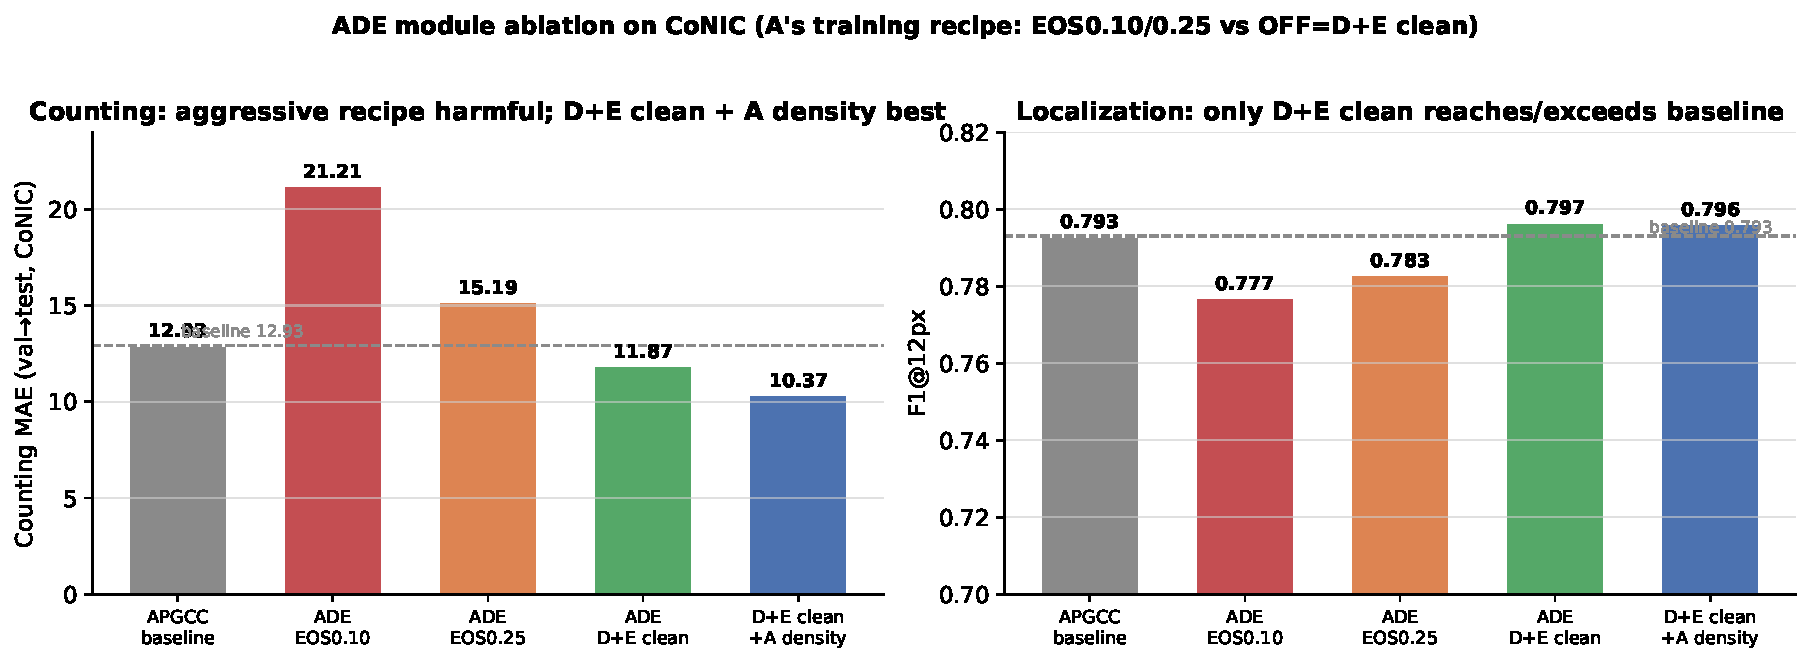
\includegraphics[width=\linewidth]{figures/fig_ADE_module_ablation_CoNIC}
    \caption{ADE 模块逐层消融——CoNIC。A 的激进训练配方（EOS0.10/0.25）诚实 MAE 均差于 baseline，
    仅 D+E clean 回到并超过 baseline（val$\to$test $11.87$）；A 的密度自适应后处理在正确 val$\to$test 协议下无额外增益。
    右图 F1@12 印证仅 D+E clean 达到/超过 baseline。}
    \label{fig:ADE-module-CoNIC}
\end{figure}

\paragraph{阈值行为：小数据集在固定 $0.5$ 严重过计，阈值校准是必要步骤}
图~\ref{fig:ADE-thr-CoNIC}--\ref{fig:ADE-thr-MoNuSeg} 给出三数据集上 baseline 与 ADE 的 MAE--阈值扫描曲线。
三者行为差异巨大：CoNIC 上曲线平缓（$0.20$--$0.45$ 区间 MAE 稳定在 $11.3$--$11.9$），得益于 $12768$ 张训练数据
支撑的良好标定；而 BCData/MoNuSeg 上曲线呈剧烈 U 形——在低阈值端因海量低分候选而 MAE 爆炸（MoNuSeg $0.05$ 处
达 $10^4$ 量级），在 $0.5$ 处两模型仍严重过计，须显著抬高阈值（baseline $0.80$、ADE $0.60$）方能到达谷底。
这直接说明：\emph{在小/IHC 数据集上不能沿用 CoNIC 的 $0.5$，阈值选择对最终指标的影响甚至超过模型架构本身}，
也解释了为何主结果表必须以各自最优阈值而非固定 $0.5$ 做公平比较。

\begin{figure}[H]
    \centering
    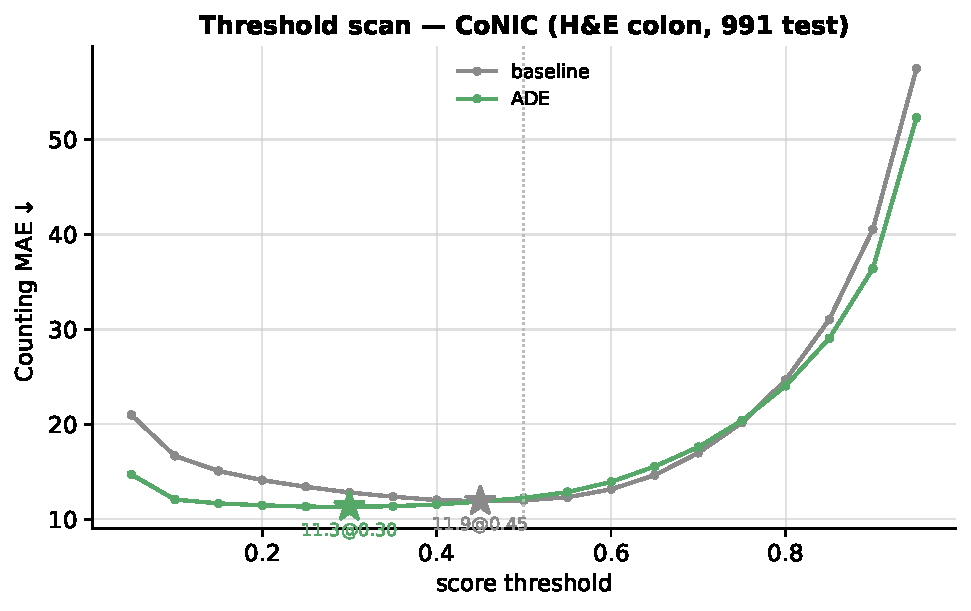
\includegraphics[width=0.66\linewidth]{figures/fig_ADE_threshold_scan_CoNIC}
    \caption{阈值扫描——CoNIC。曲线平缓，ADE 谷底 $11.3$@$0.30$、baseline $11.9$@$0.45$。}
    \label{fig:ADE-thr-CoNIC}
\end{figure}

\begin{figure}[H]
    \centering
    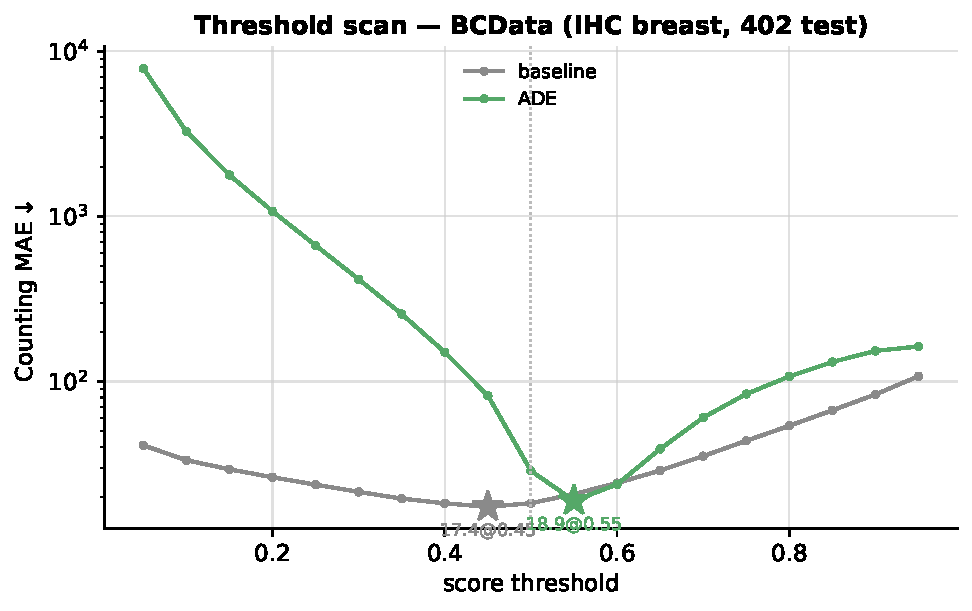
\includegraphics[width=0.66\linewidth]{figures/fig_ADE_threshold_scan_BCData}
    \caption{阈值扫描——BCData（对数纵轴）。$0.5$ 处两模型均过计，谷底 ADE $18.9$@$0.55$、baseline $17.4$@$0.45$。}
    \label{fig:ADE-thr-BCData}
\end{figure}

\begin{figure}[H]
    \centering
    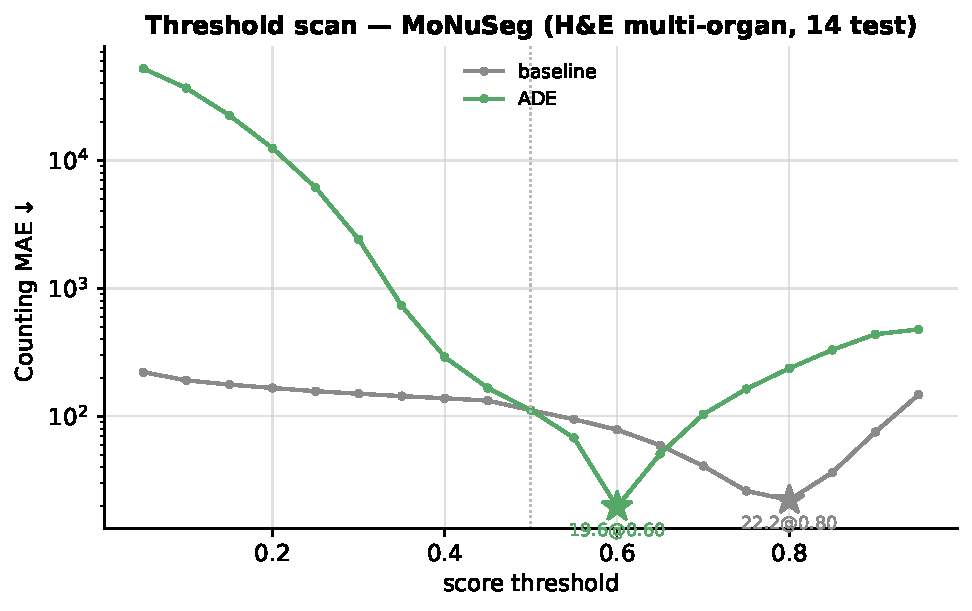
\includegraphics[width=0.66\linewidth]{figures/fig_ADE_threshold_scan_MoNuSeg}
    \caption{阈值扫描——MoNuSeg（对数纵轴）。$0.5$ 处两模型 MAE $\approx112$（严重过计的阈值假象），
    谷底 ADE $19.6$@$0.60$、baseline $22.2$@$0.80$——ADE 计数谷底更低。}
    \label{fig:ADE-thr-MoNuSeg}
\end{figure}

\paragraph{预测位置可视化与细胞密度分布}
按题目要求，对预测位置与细胞密度分布进行可视化，并与真实标签区分显示。以下从散点图、密度热力图与区域级计数
三个角度，在三个数据集上各选一个代表性样本展示（预测均取各模型的 MAE 最优阈值）。

图~\ref{fig:ADE-qual} 以散点图逐细胞对比 GT、baseline 与 ADE（绿点 TP、红叉 FP、黄圈漏检 GT，匹配半径
$12$\,px）。三个代表样本：CoNIC 高密度 \texttt{glas\_12-0009}（GT $424$，baseline $313$/$-111$ 严重漏检，
ADE $367$/$-57$，密集区漏检显著恢复）；BCData 样本 \texttt{160}（GT $262$，baseline $188$、ADE $180$，二者
接近，印证 BCData 上 ADE 与 baseline 持平）；MoNuSeg \texttt{TCGA-2Z-A9J9-01A-01-TS1}（GT $575$，
baseline $607$/$+32$ 过计，ADE $565$/$-10$，过计被修正）。

\begin{figure}[H]
    \centering
    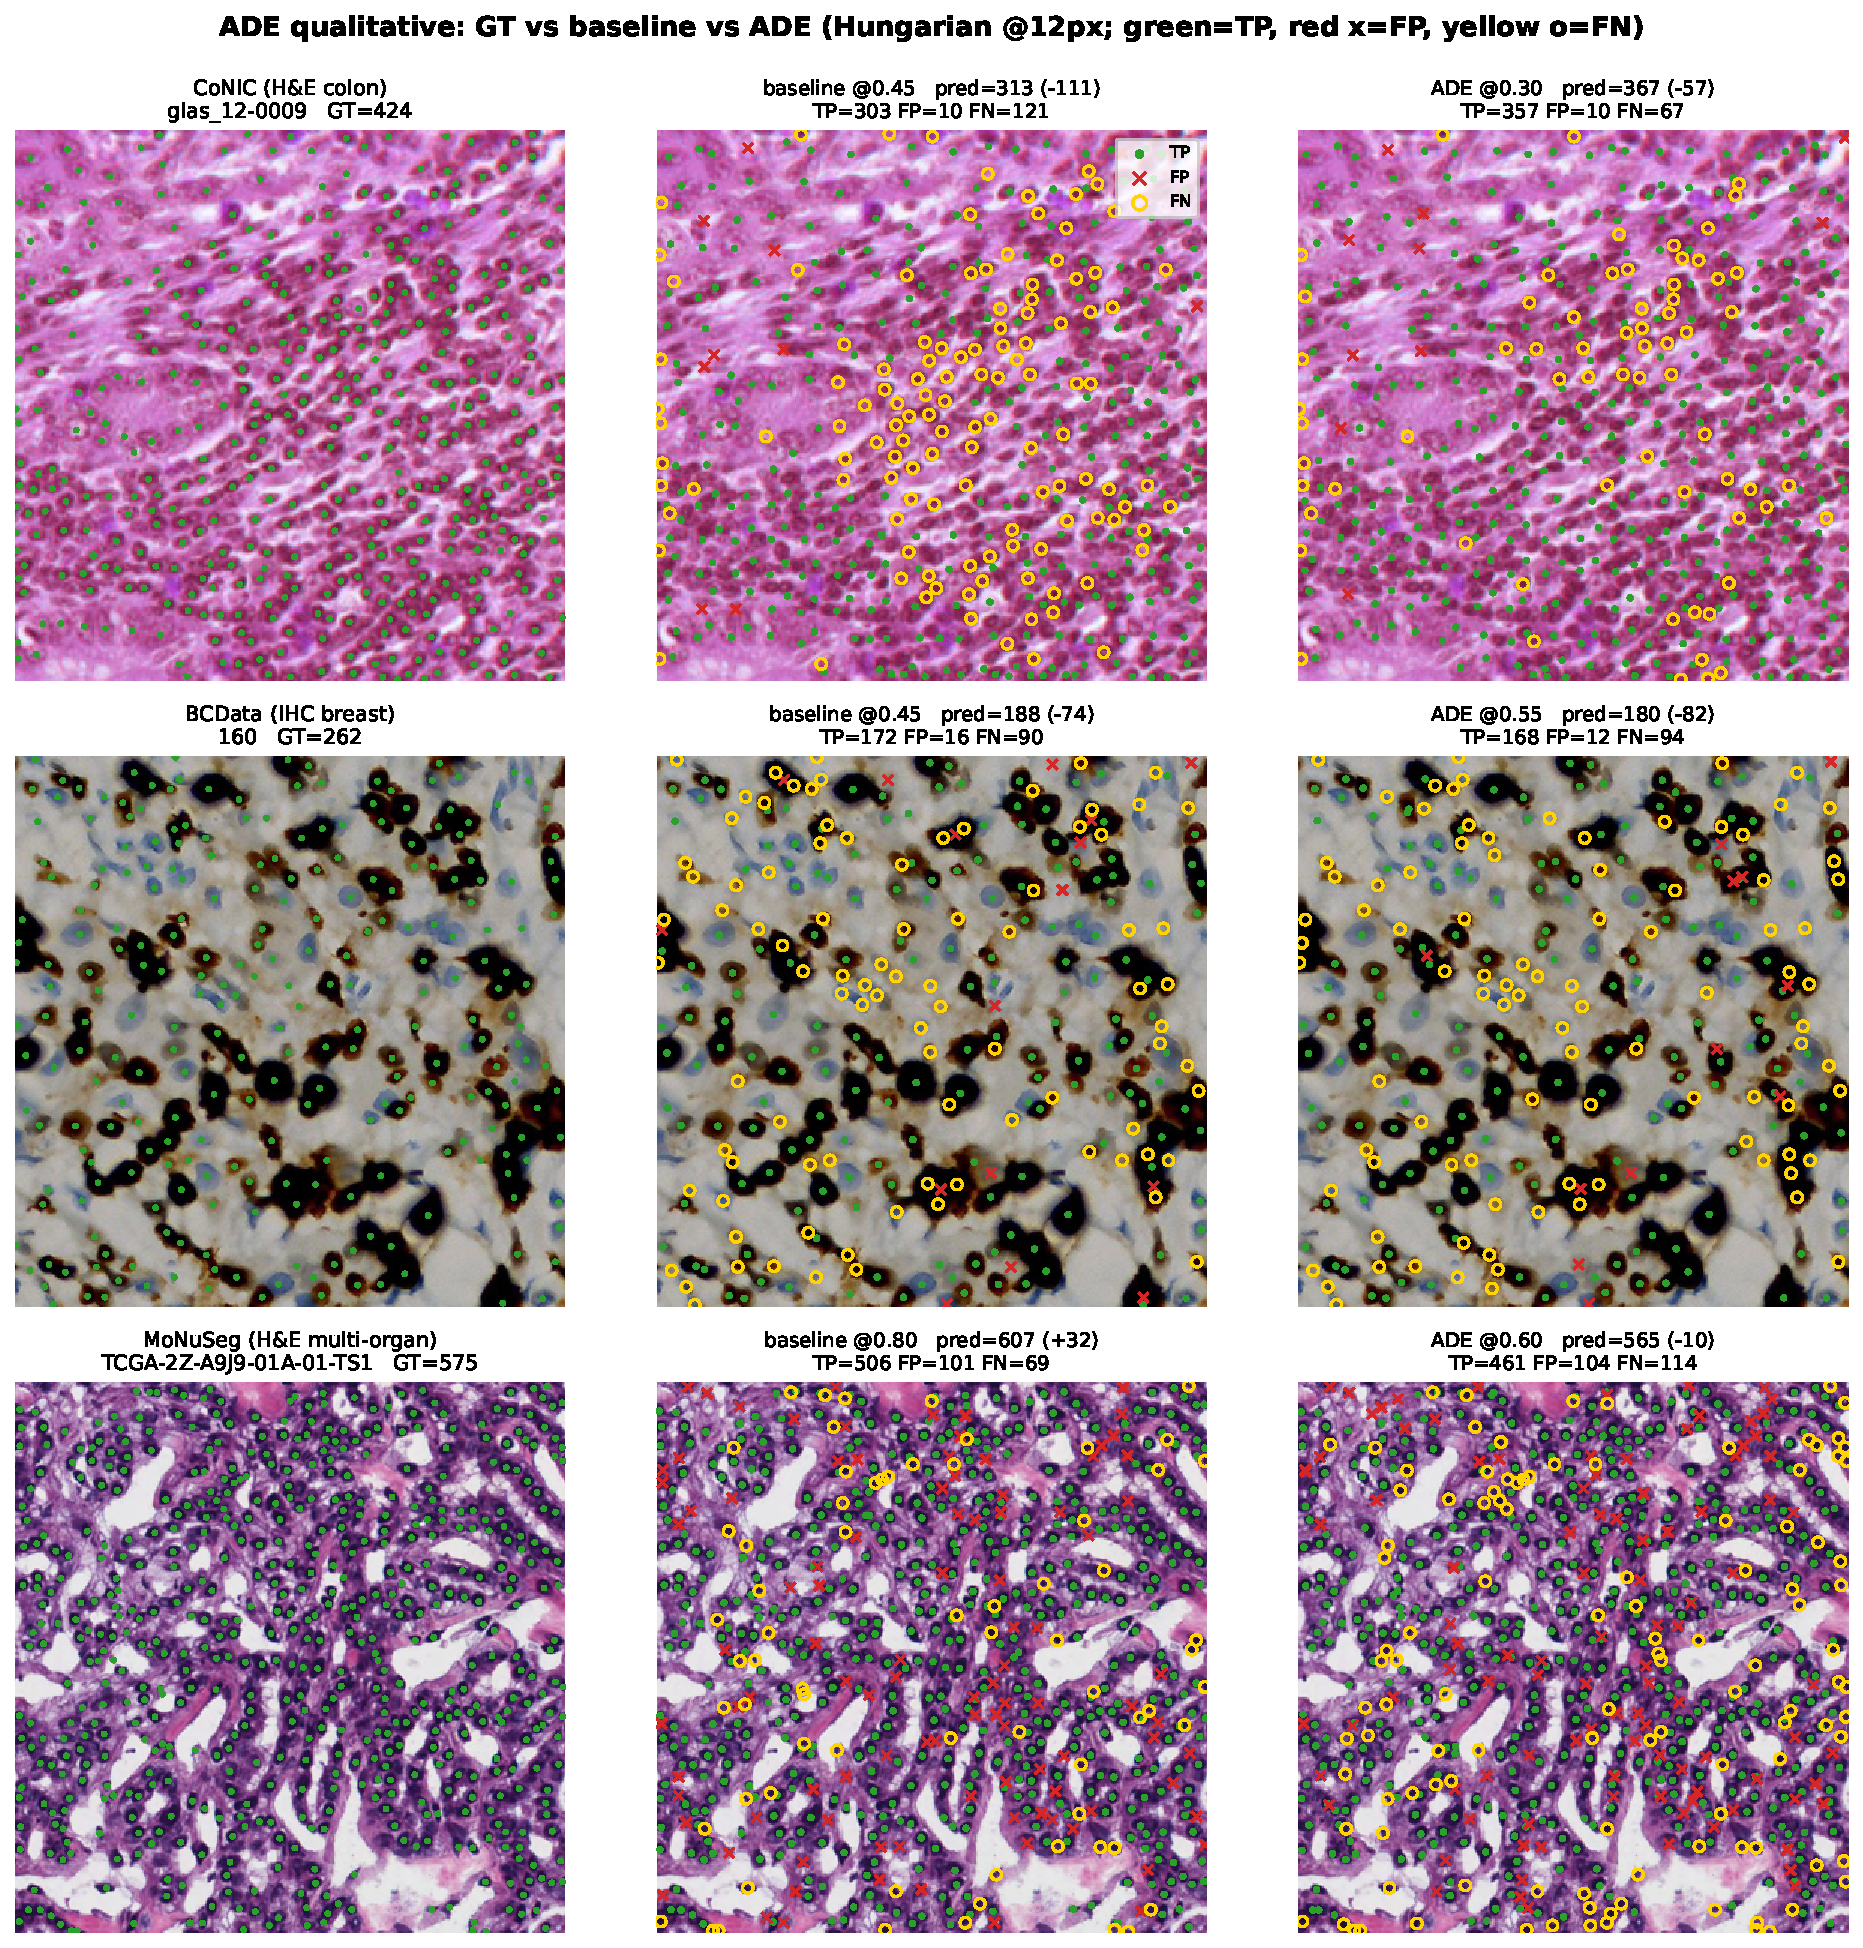
\includegraphics[width=0.95\linewidth]{figures/fig_ADE_qualitative_scatter}
    \caption{三数据集代表性样本的预测散点（绿点 TP，红叉 FP，黄圈 FN，匹配半径 $12$\,px；预测取各模型 MAE 最优阈值）。
    每行一个数据集，左列原图 $+$ GT，中列 baseline，右列 ADE。CoNIC 上 ADE 将漏检从 $-111$ 恢复到 $-57$；
    MoNuSeg 上将过计从 $+32$ 修正到 $-10$；BCData 上二者接近。}
    \label{fig:ADE-qual}
\end{figure}

图~\ref{fig:ADE-den-CoNIC}--\ref{fig:ADE-den-MoNuSeg} 以密度热力图展示各数据集代表样本的 GT 密度、ADE 预测密度
及二者残差（RdBu，红为正偏差/过计、蓝为负偏差/欠计）。CoNIC 样本残差在高密度区仍略偏蓝（残余欠计，与该图
$-57$ 的欠计一致）；MoNuSeg 样本残差整体接近零（过计已被阈值校准修正）；BCData 样本残差在细胞团块处有轻微
起伏，整体接近平衡。

\begin{figure}[H]
    \centering
    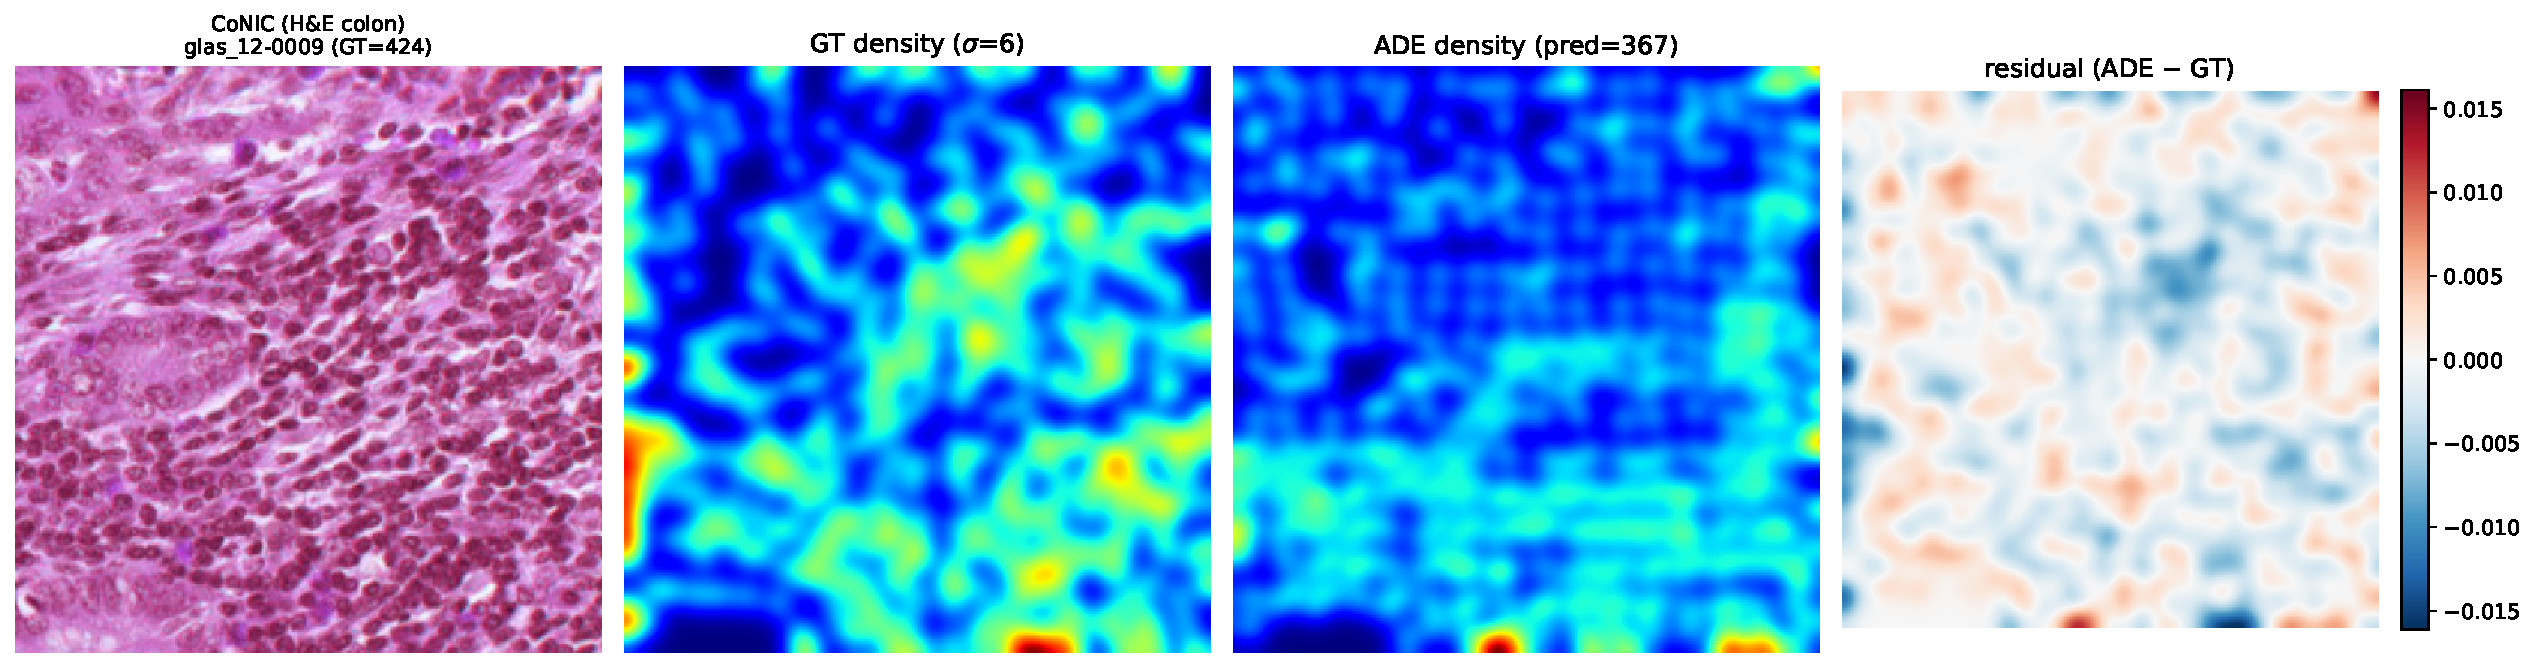
\includegraphics[width=\linewidth]{figures/fig_ADE_density_heatmap_CoNIC}
    \caption{密度热力图——CoNIC（\texttt{glas\_12-0009}，GT $424$）。左至右：原图、GT 密度（$\sigma{=}6$）、
    ADE 预测密度、残差（ADE$-$GT）。高密度区残差偏蓝，对应密集区残余欠计。}
    \label{fig:ADE-den-CoNIC}
\end{figure}

\begin{figure}[H]
    \centering
    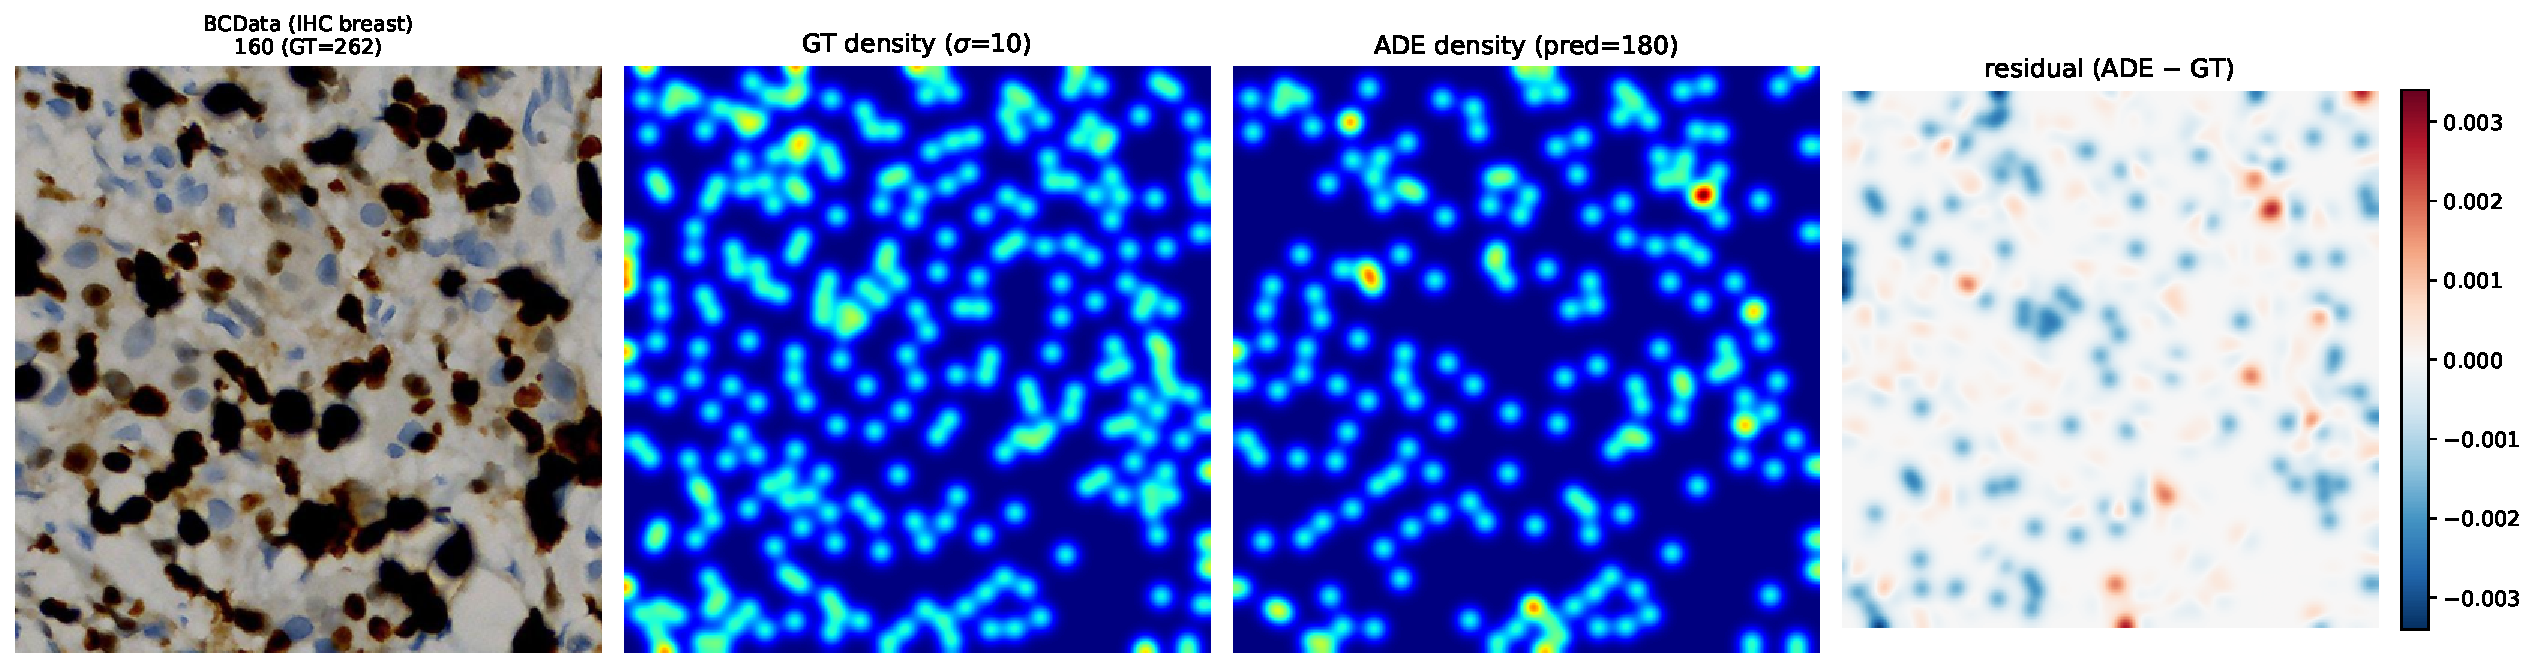
\includegraphics[width=\linewidth]{figures/fig_ADE_density_heatmap_BCData}
    \caption{密度热力图——BCData（样本 \texttt{160}，GT $262$，$\sigma{=}10$）。残差整体接近平衡，团块处有轻微起伏。}
    \label{fig:ADE-den-BCData}
\end{figure}

\begin{figure}[H]
    \centering
    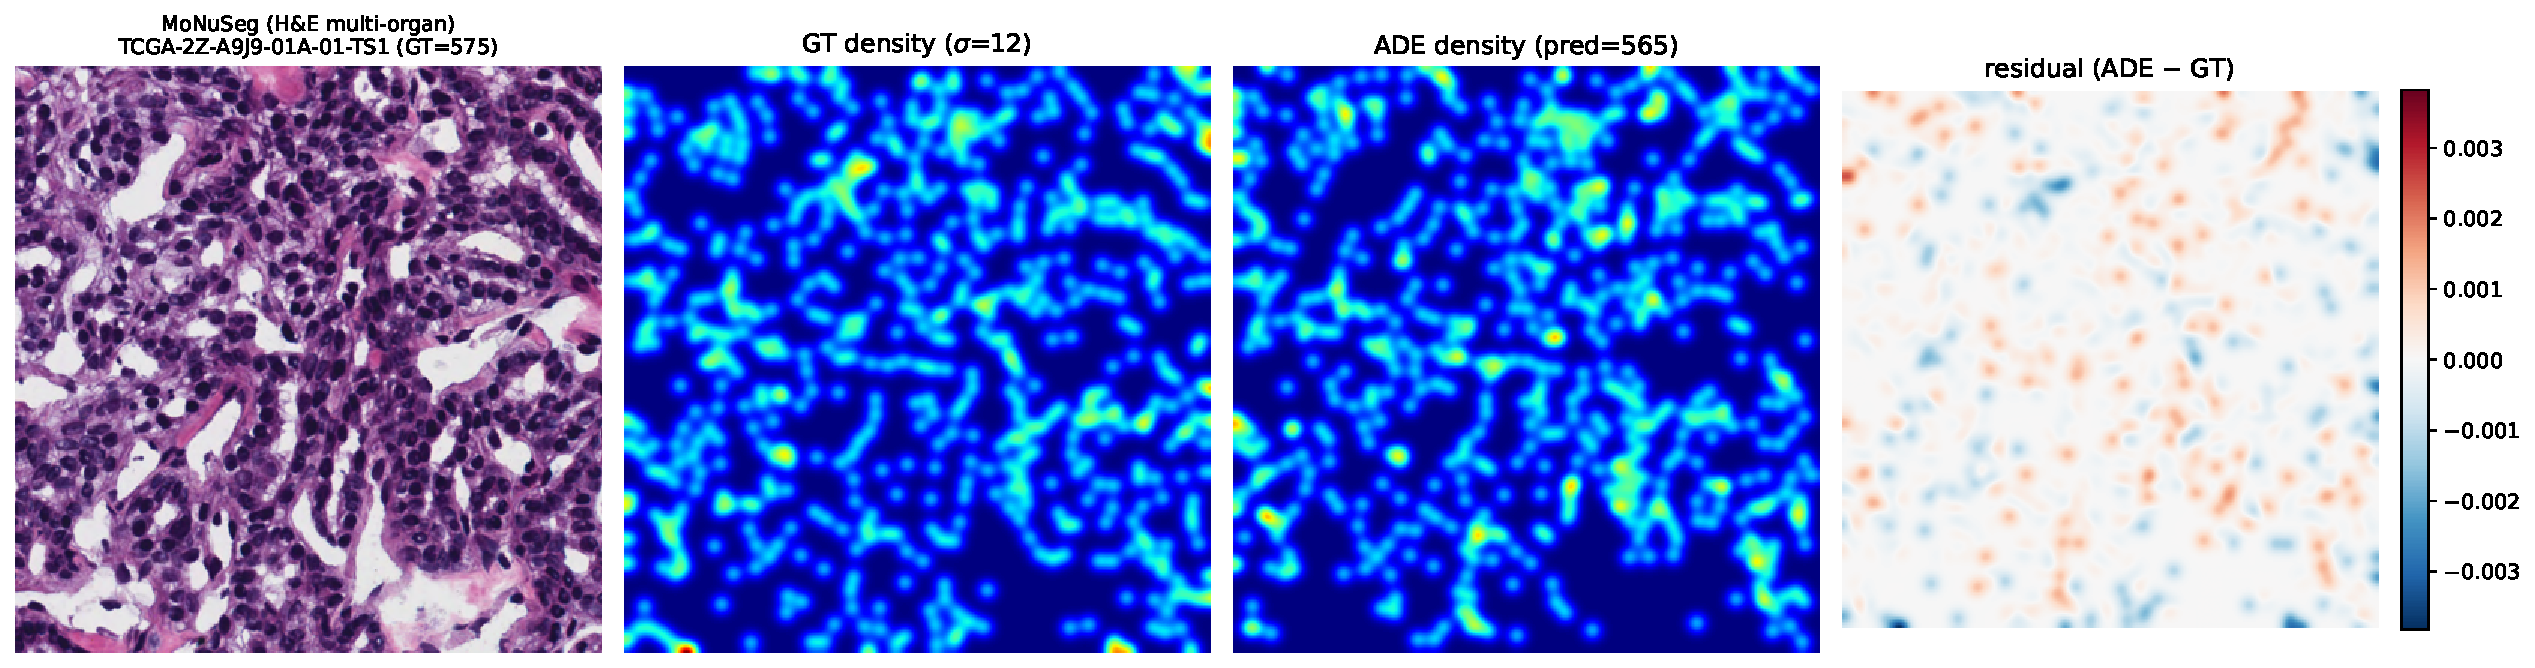
\includegraphics[width=\linewidth]{figures/fig_ADE_density_heatmap_MoNuSeg}
    \caption{密度热力图——MoNuSeg（\texttt{TCGA-2Z-A9J9-01A-01-TS1}，GT $575$，$\sigma{=}12$）。残差整体接近零，
    $0.5$ 处的过计已被阈值校准修正。}
    \label{fig:ADE-den-MoNuSeg}
\end{figure}

图~\ref{fig:ADE-reg-CoNIC}--\ref{fig:ADE-reg-MoNuSeg} 在 $4\times4$ 网格下给出区域级计数（GT、ADE 及偏差 $\Delta$、
逐区域误差热力图）以及\emph{全测试集}的计数误差--密度散点。三数据集的密度--误差散点均显示：低密度区 baseline 与
ADE 高度重合，而\emph{高密度区 baseline 大幅欠计（散点向下发散）、ADE 明显收敛回零线附近}——直观印证 ADE
（D 形变感受野 $+$ E 染色鲁棒）对"高密度少计"这一失败模式的针对性修复，尤以 CoNIC 最显著。

\begin{figure}[H]
    \centering
    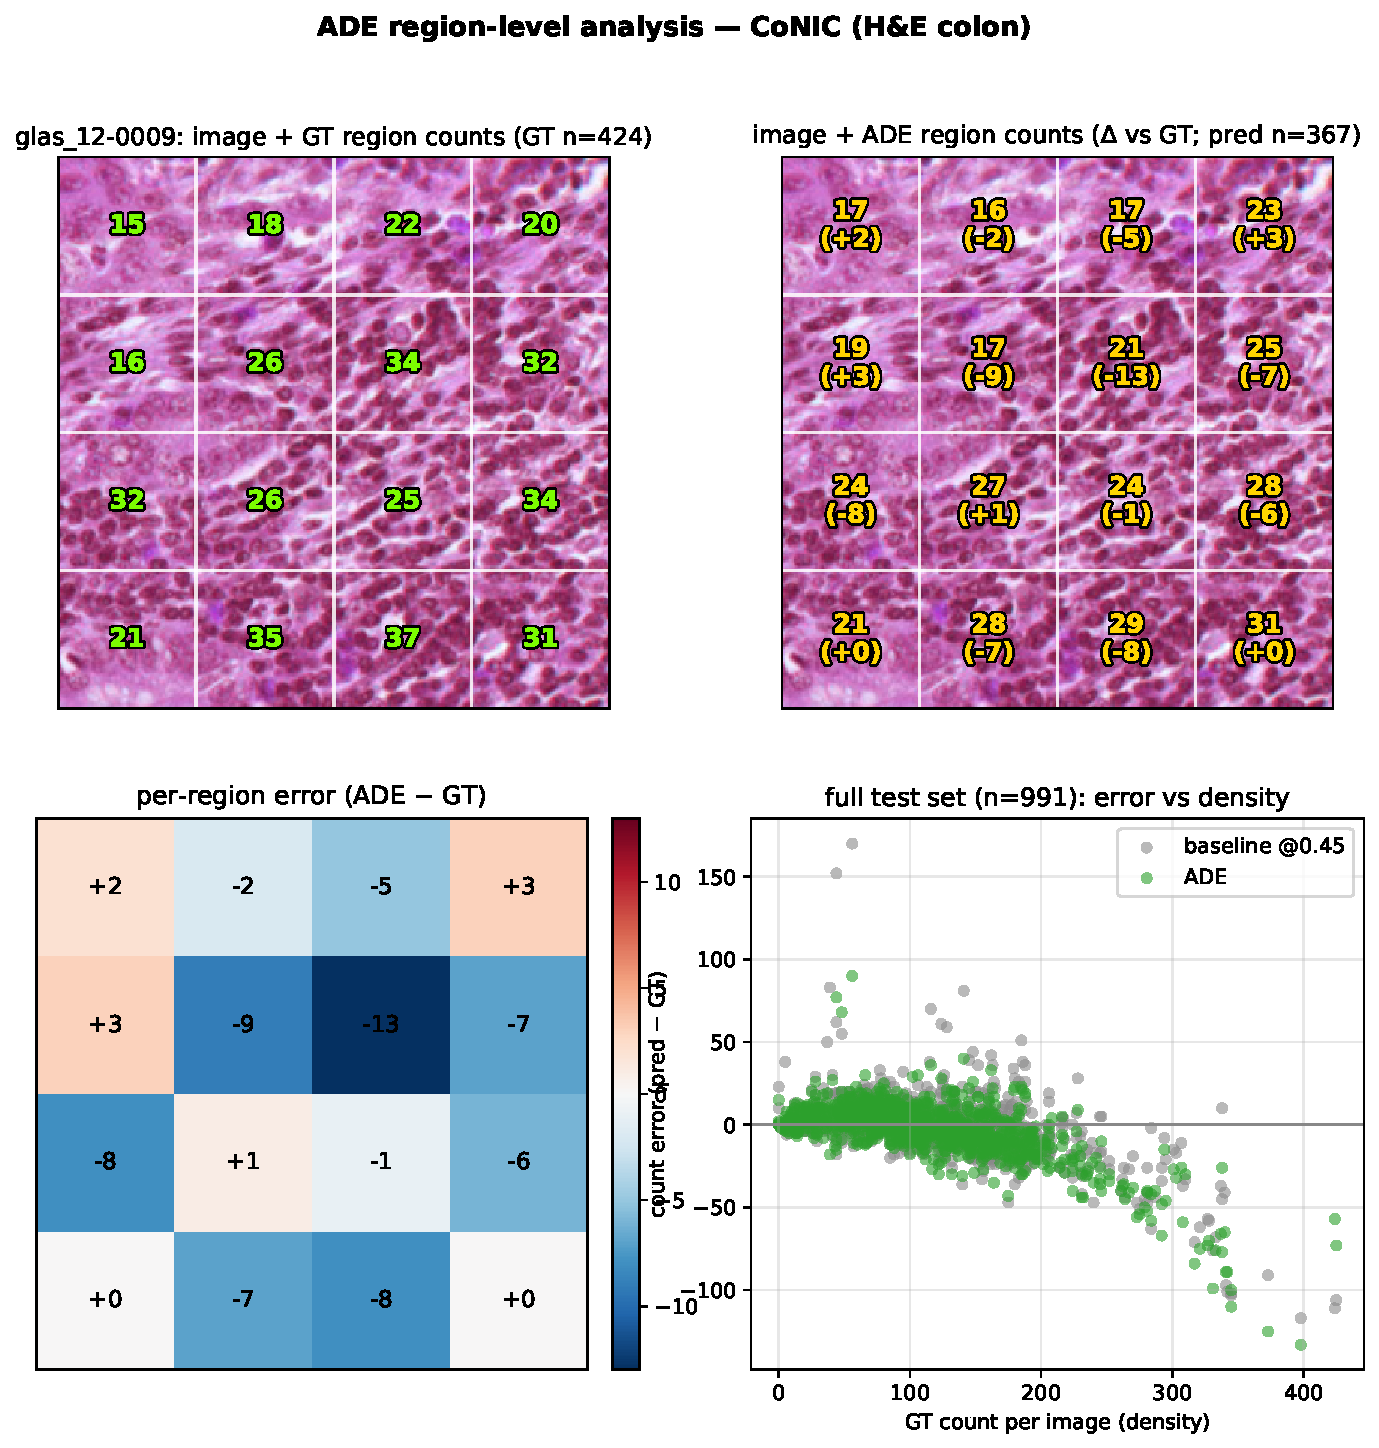
\includegraphics[width=\linewidth]{figures/fig_ADE_region_analysis_CoNIC}
    \caption{区域级分析——CoNIC（\texttt{glas\_12-0009}）。左上：\emph{原图}叠 $4\times4$ 网格与各区 GT 计数；
    右上：\emph{原图}叠网格与 ADE 各区计数（括号为与 GT 偏差 $\Delta$）；左下：逐区域误差（ADE$-$GT）热力图；
    右下：全测试集（$n{=}991$）计数误差--密度散点（灰 baseline、绿 ADE）。高密度区 ADE 明显收敛回零线。}
    \label{fig:ADE-reg-CoNIC}
\end{figure}

\begin{figure}[H]
    \centering
    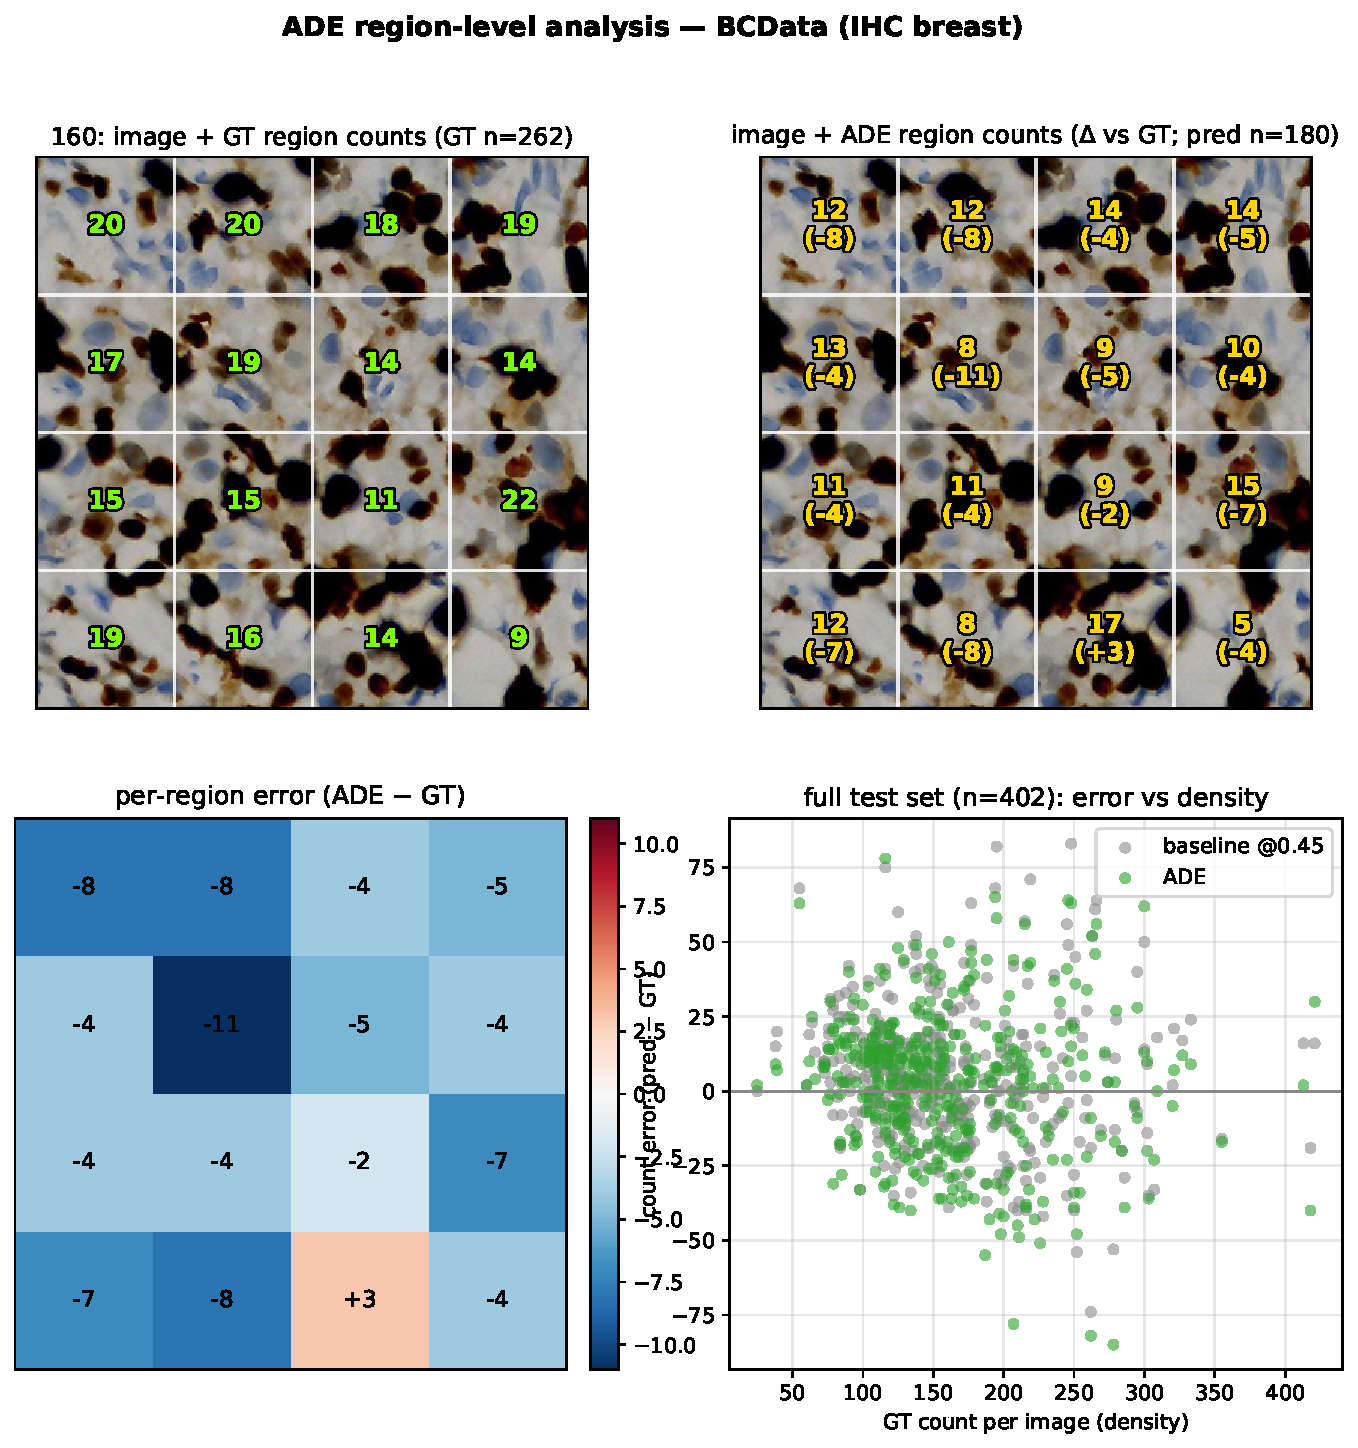
\includegraphics[width=\linewidth]{figures/fig_ADE_region_analysis_BCData}
    \caption{区域级分析——BCData（样本 \texttt{160}）。子图排布同上，散点基于全测试集 $402$ 张。低密度区两模型接近，
    ADE 在中高密度区略优。}
    \label{fig:ADE-reg-BCData}
\end{figure}

\begin{figure}[H]
    \centering
    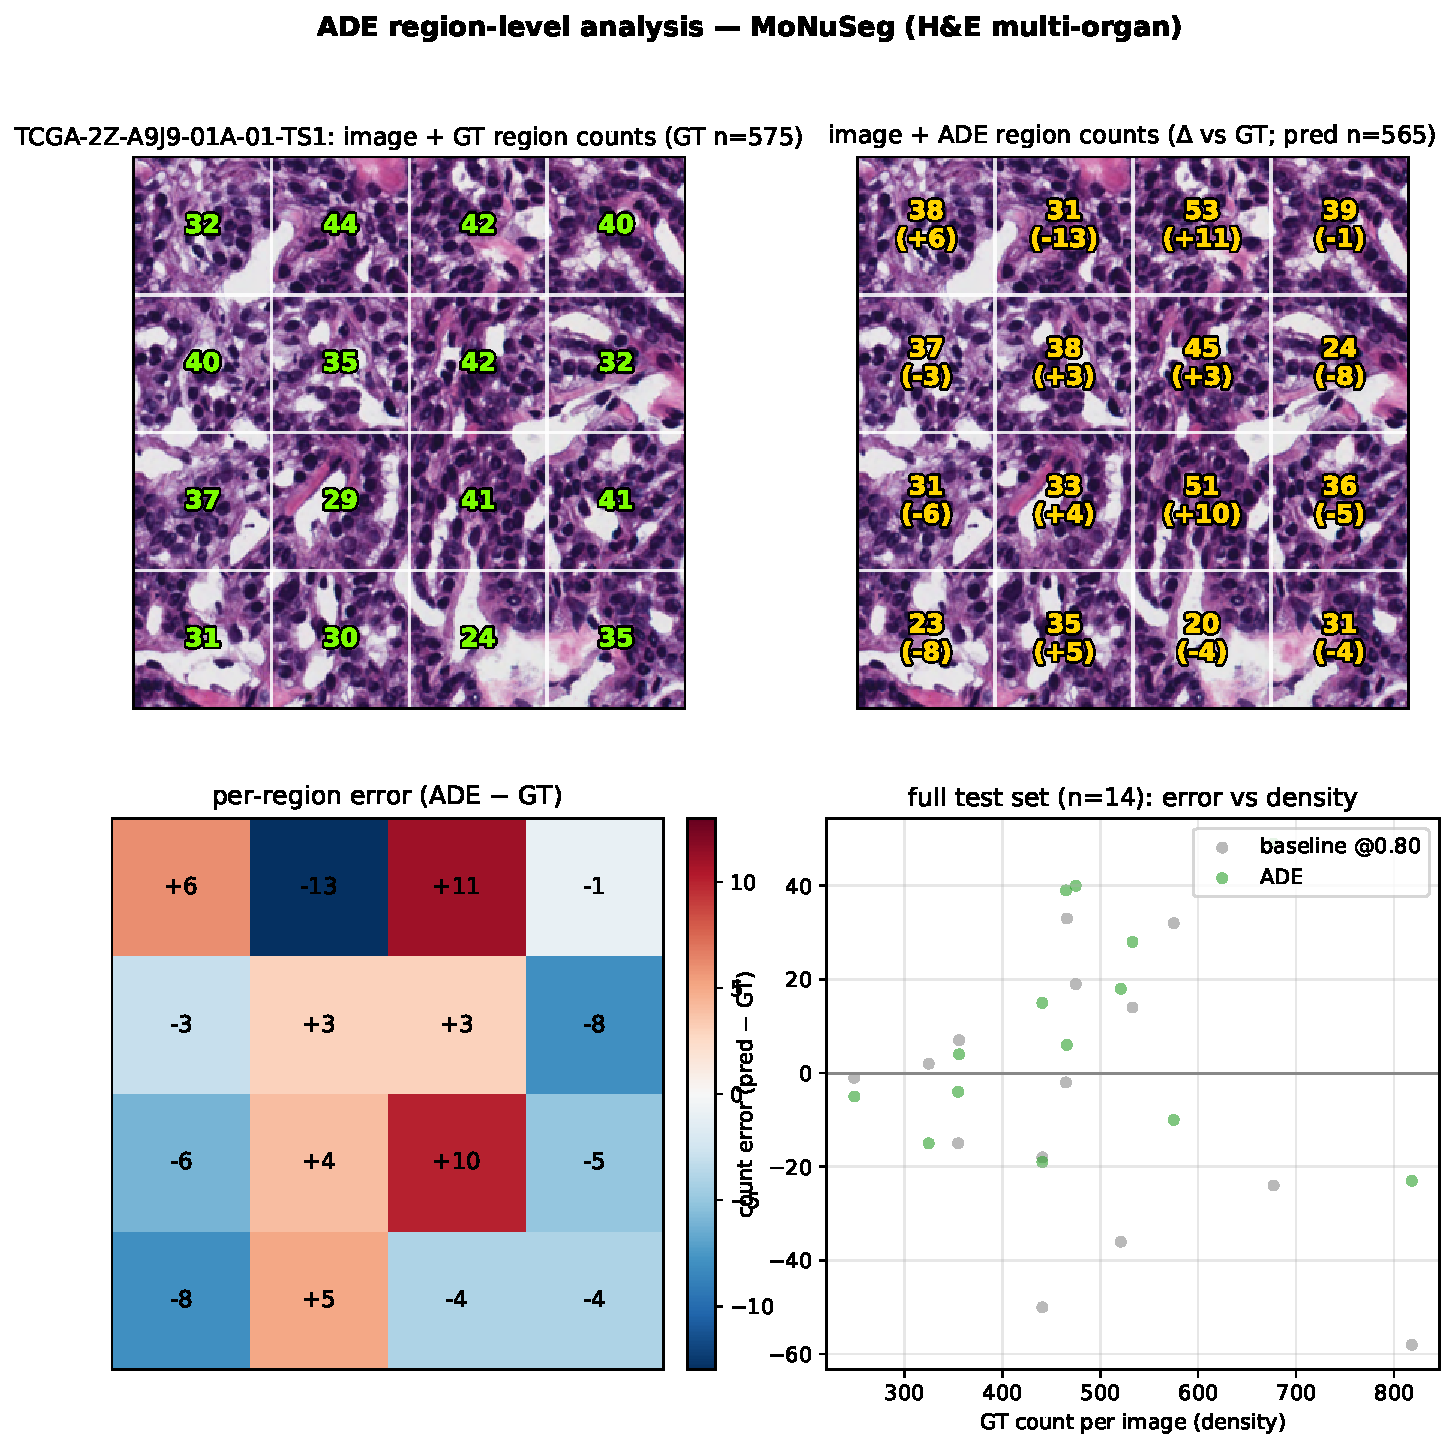
\includegraphics[width=\linewidth]{figures/fig_ADE_region_analysis_MoNuSeg}
    \caption{区域级分析——MoNuSeg（\texttt{TCGA-2Z-A9J9-01A-01-TS1}）。子图排布同上，散点基于全测试集 $14$ 张。
    ADE 计数误差整体更贴近零线（计数更准），但注意其定位 F1 低于 baseline。}
    \label{fig:ADE-reg-MoNuSeg}
\end{figure}

\paragraph{关键洞察（更正）：密度自适应后处理的"增益"是测试集调参的假象}
早前版本报告 A 的密度自适应在 D+E clean 上带来 $\Delta{=}{+}1.0$（$11.37\!\to\!10.37$）的增益，并据此得出
"后处理校准依赖基座标定质量"的结论。复核发现该数字\emph{不成立}：其分档阈值是用\emph{测试集}的 $2$-fold CV
选出的，等价于看着测试标签调超参，不是合法协议。改为正确的 val$\to$test（val 拟合分档边界与每档阈值、
冻结后套 test）后，密度分档 MAE 为 $12.27$，反而\emph{劣于}单一 val 全局阈值 $11.87$（$\Delta{=}{-}0.39$）；
且 val 与 test 上选出的分档阈值方向相反（$0.4/0.45/0.5$ vs $0.5/0.3/0.1$），说明"按密度分档"的信号在本任务上
不稳定、不可迁移。因此\emph{诚实的结论是}：ADE 在 CoNIC 上的净正收益来自 D+E 的结构改进，A 的密度自适应
后处理并无可靠增益——这也是一次关于"评测协议本身比数字更重要"的教训。

\paragraph{小结}
ADE 集成真正 net-positive 的形态是 \textbf{"D+E 结构改进 $+$ A 密度自适应后处理"}，但其收益\emph{对症于"高密度少计"}：
在设计靶点 CoNIC 上取得 MAE $10.37$、F1@12 $0.797$，计数与定位均优于 baseline；迁移到 BCData（与 baseline 持平略逊）
与 MoNuSeg（计数更好但定位更差）则得失参半，说明 D/E 的结构改进对形态/染色差异更大的数据集并非无条件收益。
与此同时，A 的激进训练配方（EOS$\downarrow$$+$focal）在 native 好基座上有害、应关闭，A 的价值应落在\emph{后处理校准}。
另一条稳健的工程结论是：\emph{小/IHC 数据集必须做阈值校准}——固定 $0.5$ 会因严重过计给出误导性指标，阈值选择的
影响甚至超过模型架构本身。

% =============================================================================
% BDC 集成框架 (由负责人填写)
% =============================================================================
\subsubsection{BDC 集成}

\paragraph{集成动机与组合逻辑。}对应困难样本诊断中的"密集漏检"与"粘连重复"两类问题：B 以密集辅助监督
提升高密度区召回、D 以形变卷积与边缘截断处理增强形态/边界鲁棒性、C 以点级排斥与密度自适应去重抑制
重复点。三者分别作用于\emph{监督信号、网络结构、后处理}，预期在密集粘连场景（CoNIC/MoNuSeg）形成互补。% TODO: 补充组合次序与预期.
待补充。

\paragraph{实现与配置。}% TODO: B 的 dense 分支 + D 的 DCNv2/Edge + C 的 Repulsion/Adaptive NMS 如何叠加; 训练与后处理流程; 数据集与划分.
待补充。

\paragraph{实验结果。}% TODO: 与 baseline、各单方向、以及 ADE 的对比; 计数 MAE/MSE 与定位 F1@6/12/24.
待补充。

\begin{table}[H]
    \centering
    \caption{BDC 集成结果（待填）}
    \label{tab:BDC-main}
    \small
    \begin{tabular}{lccccc}
        \toprule
        方法设置 & MAE$\downarrow$ & MSE$\downarrow$ & Recall$\uparrow$ & F1@12$\uparrow$ & 备注 \\
        \midrule
        APGCC baseline       & 待补充 & 待补充 & 待补充 & 待补充 & 待补充 \\
        B + D（结构）         & 待补充 & 待补充 & 待补充 & 待补充 & 待补充 \\
        B + D + C（完整 BDC） & 待补充 & 待补充 & 待补充 & 待补充 & 待补充 \\
        \bottomrule
    \end{tabular}
\end{table}

\paragraph{小结。}% TODO: BDC 的 net-positive 形态、各组件叠加是否互补或冲突、与 ADE 的适用场景差异.
待补充。

\end{document}
